% !TeX spellcheck = pt_BR
\documentclass[tese_patricia]{subfiles}
\begin{document}

% ---------------------------------------------------------- 
% Métodos de malhas sobrepostas
% ----------------------------------------------------------
\chapter[Análise isogeométrica aplicada à Dinâmica dos Fluidos Computacional]{Análise isogeométrica aplicada à Dinâmica dos Fluidos Computacional} \label{capitulo:Cap3}
% ----------------------------------------------------------

%\nomenclature[C,01]{$p$}{Grau das funções base na direção paramétrica $\xsi$;}
%\nomenclature[C,02]{$\xsi$}{Vetor de \textit{knots} na direção paramétrica $\xsi$;}
%\nomenclature[C,03]{$\xsi$}{Uma das direções paramémtricas nas quais as funções base são definidas;}
%\nomenclature[C,04]{$n$}{Número de funções base na direção paramétrica $\xsi$ ;}
%\nomenclature[C,05]{$N$}{Função base \textit {B-Spline} na direção paramétrica $\xsi$ ;}
%\nomenclature[C,06]{$\CP$}{Pontos de controle que descrevem a geometria \textit{B-Spline} ou NURBS;}
%\nomenclature[C,07]{$\mathbf{C}$}{Curva \textit {B-Spline} ou NURBS;}
%\nomenclature[C,08]{$m$}{Grau das funções base na direção paramétrica $\eta$;}
%\nomenclature[C,09]{$\mathcal{H}$}{Vetor de \textit{knots} na direção paramétrica $\eta$;}
%\nomenclature[C,10]{$q$}{Número de funções base na direção paramétrica $\eta$ ;}
%\nomenclature[C,11]{$\eta$}{Uma das direções paramémtricas nas quais as funções base são definidas;}
%\nomenclature[C,12]{$M$}{Função base \textit {B-Spline} na direção paramétrica $\eta$ ;}
%\nomenclature[C,13]{$\mathbf{S}$}{Superfície \textit {B-Spline} ou NURBS;}
%\nomenclature[C,14]{$\hat{N}$}{Função \textit {B-Spline} fruto do produto tensorial entre funções base descritas em um espaço paramétrico qualquer;}
%\nomenclature[C,15]{$L$}{Função base \textit {B-Spline} na direção paramétrica $\zeta$ ;}
%\nomenclature[C,16]{$r$}{Grau das funções base na direção paramétrica $\zeta$;}
%\nomenclature[C,17]{$\mathcal{Z}$}{Vetor de \textit{knots} na direção paramétrica $\zeta$;}
%\nomenclature[C,18]{$\zeta$}{Uma das direções paramémtricas nas quais as funções base são definidas;}
%\nomenclature[C,19]{$l$}{Número de funções base na direção paramétrica $\zeta$ ;}
%\nomenclature[C,20]{$\mathbf{T}$}{Sólido \textit {B-Spline} ou NURBS;}
%\nomenclature[C,21]{$\mathbf{C}^{w}$}{Curva \textit{B-Spline} no $\realspace^{d+1}$ cuja projeção transformativa gera uma curva \mathbf{C} no $\realspace^{d}$;}
%\nomenclature[C,22]{$R$}{Função base NURBS;}
%\nomenclature[C,23]{$w$}{Peso respectivo a um ponto de controle;}
%\nomenclature[C,24]{$\mathbf{\hat{\xsi}}$}{Coordenadas do espaço parental, no qual realiza-se a integração numérica;}
%\nomenclature[C,25]{$\hat{\xsi}$}{Uma das direções do espaço parental;}
%\nomenclature[C,26]{$\hat{\eta}$}{Uma das direções do espaço parental;}
%\nomenclature[C,27]{$\hat{\zeta}$}{Uma das direções do espaço parental;}
%\nomenclature[C,28]{$\tilde{\Omega^{e}}$}{Domínio de uma célula no espaço paramétrico;}
%\nomenclature[C,29]{$\hat{\Omega^{e}}$}{Domínio de um uma célula o no espaço parental;}
%\nomenclature[C,30]{$h$}{Dimensão na direção $y$ da entrada do perfil parabólico no problema do escoamento sobre canal com degrau;}
%\nomenclature[C,31]{$s$}{Dimensão  na direção $y$ do degrau que compõe o problema do escoamento sobre canal com degrau;}
%\nomenclature[C,32]{$x_{e}$}{Dimensão na direção $x$  do degrau que compõe o problema do escoamento sobre canal com degrau;}
%\nomenclature[C,33]{$x_{f}$}{Dimensão na direção $x$  do \textit{patch} $P1$ do problema do escoamento sobre canal com degrau;}
%\nomenclature[C,34]{$x_{t}$}{Dimensão do canal após o degrau na direção $x$ do problema do escoamento sobre canal com degrau;}
%\nomenclature[C,35]{$V_{max}$}{Velocidade máxima do perfil parabólico na entrada do problema do escoamento sobre canal com degrau;}
%\nomenclature[C,36]{$x_{r}$}{Dimensão do vórtice primário que se forma no problema de escoamento sobre canal com degrau;}
%\nomenclature[C,37]{$P_{i}$}{Patch de número $i$;}


A Análise Isogeométrica (IGA) é uma técnica numérica introduzida por \citeonline{HughesCB:2005} para obtenção de soluções aproximadas de equações diferenciais. O método pode ser entendido como uma generalização do método dos elementos finitos clássicos a partir do uso de funções base especiais. 

Na Análise Isogeométrica, as funções base escolhidas na discretização da geometria do problema e de suas variáveis são aquelas utilizadas nos sistemas CAD, sendo as funções do tipo NURBS as mais aplicadas (ver, por exemplo, \citeonline{PiegT:1996}). O grande impulso para o desenvolvimento da técnica foi proporcionar a integração entre a engenharia de \textit{design}, com modelos baseados em CAD, e as simulações numéricas, com modelos principalmente baseados no MEF, de forma que ambas trabalhem com somente um modelo geométrico.

A IGA apresenta vantagens significativas, uma vez que permite a representação exata de diversas geometrias comuns, como seções cônicas, círculos, cilindros, esferas e elipsoides, além de dispor de algoritmos eficientes e estáveis para a geração de objetos NURBS. As funções NURBS, em particular, possuem propriedades matemáticas que as tornam adequadas para aplicações numéricas, destacando-se a elevada suavidade, a alta capacidade de aproximação e a possibilidade de refinamento local por meio da inserção de \textit{knots}, os quais correspondem às coordenadas do espaço paramétrico nas quais as funções são definidas.

Este capítulo apresenta uma breve introdução à Análise Isogeométrica (IGA) e sua relação com o Método dos Elementos Finitos clássico. Inicialmente, são descritas as funções base B-spline, suas principais características e a construção de geometrias associadas. Em seguida, introduzem-se as funções NURBS, destacando sua formulação e aplicações geométricas. A análise isogeométrica é então introduzida no contexto da dinâmica dos fluidos computacional, enfatizando suas particularidades quanto à discretização das variáveis e da geometria, aos métodos de integração numérica e à determinação dos parâmetros de estabilização. Por fim, são apresentados exemplos numéricos que validam a formulação proposta. As referências bibliográficas que fundamentam esta construção são \citeonline{HughesCB:2005} e \citeonline{PiegT:1996}. 

%\vspace{-0.1cm}

\section{Noções Gerais de IGA}

No contexto do MEF isoparamétrico, a formulação é construída a partir da definição de uma malha e de seus elementos, os quais são representados tanto no espaço físico quanto no espaço paramétrico. Cada elemento é caracterizado pelas coordenadas de seus nós, sendo os graus de liberdade do problema associados aos valores das funções de forma interpolados nesses pontos nodais.

Dentro da IGA têm-se duas noções de malha: uma malha de pontos de controle e uma malha física. A malha de pontos de controle é muito semelhante a uma malha de elementos finitos, entretanto, ela não define a geometria, ela é apenas um esqueleto que controla o formato da geometria (ver Fig. \ref{fig:espacos_NURBS}), visto que as funções de forma baseadas em \textit{B-Splines} não são necessariamente interpolatórias. Dessa forma, os graus de liberdade do problema são associados aos pontos de controle, cujas posições não coincidem, necessariamente, com a geometria representada.

\begin{figure}[htb!]
	\centering 
	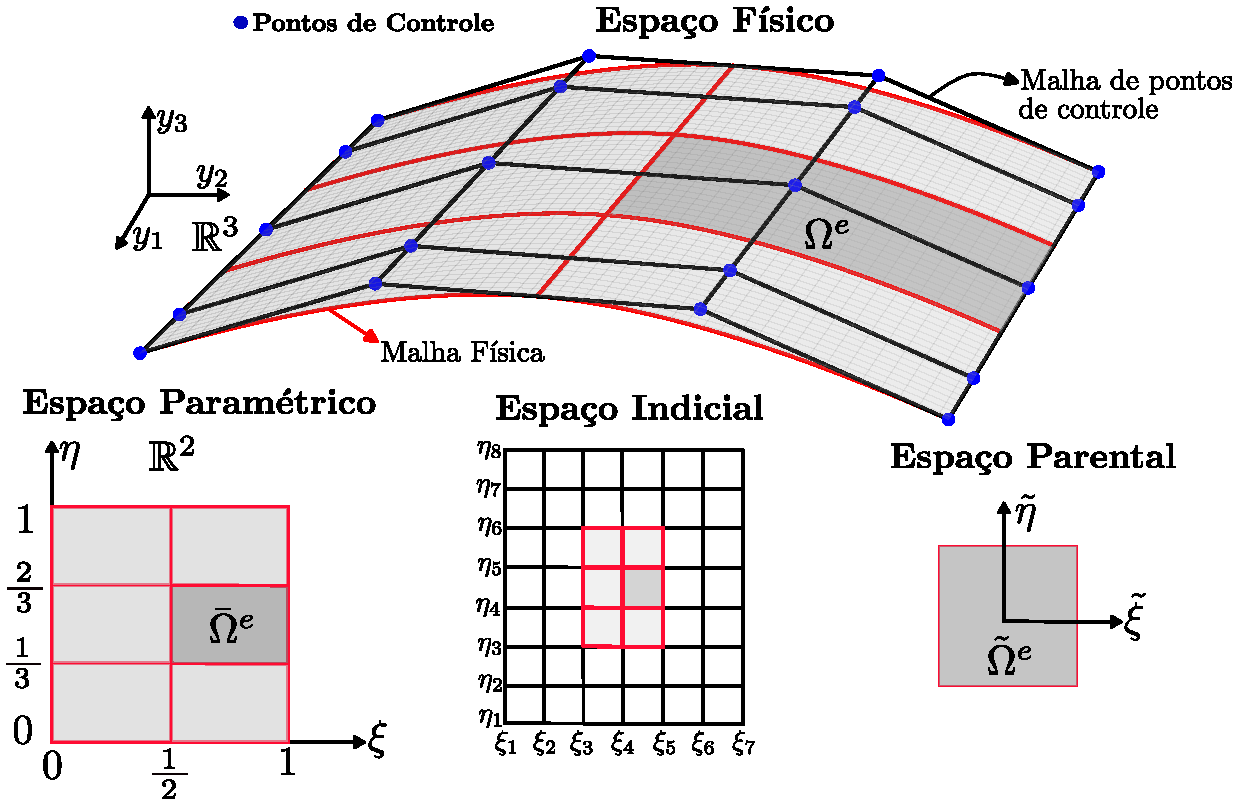
\includegraphics[scale=0.7,trim=0cm 0cm 0cm 0cm, clip=true]{Imagens/Cap3/espacos_NURBS.pdf}	
	\caption{NURBS: espaço físico, espaço paramétrico, espaço indicial e espaço parental}
	\label{fig:espacos_NURBS}
\end{figure}


A malha física representa a geometria discretizada. Dentro da malha física podem ser definidos dois tipos de elementos, um macro-elemento, denominado de \textit{patch}, e o \textit{knot span}, que é o equivalente a um elemento finito e será denominado como célula ao longo desse texto. Cada \textit{patch} é composto por um conjunto de células. Muitas geometrias simples podem ser discretizadas apenas com um \textit{patch}, entretanto, a depender da complexidade da geometria ou de requisitos de parametrização, se torna necessário o uso de um conjunto de \textit{patches}. As células são representações geométricas de linhas, superfícies e volumes nos espaços físicos unidimensional, bidimensional e tridimensional respectivamente.

Cada \textit{patch} e suas respectivas células possuem uma representação no espaço paramétrico (Fig. \ref{fig:espacos_NURBS}), que é o espaço onde as funções base são definidas. O espaço paramétrico, para os casos de funções univariadas, é definido por um \textit{knot vector}, aqui denominado de vetor de \textit{knots}, que é um conjunto de \textit{knots} ou coordenadas paramétricas. As células são constituídas pelo espaço entre dois \textit{knots} consecutivos. O espaço onde se representam todas as células, inclusive as nulas (quando mais de um \textit{knot} ocupa a mesma posição), é chamado de espaço indicial.

Por fim, na análise isogeométrica conta-se ainda com o espaço parental, que é o espaço de integração numérica das funções base, em geral, definido de forma adimensional $[-1, 1]$ dentro de uma célula. Na Fig. \ref{fig:espacos_NURBS} pode-se observar os espaços relatados para uma superfície 3D construída por funções base quadráticas e apenas um \textit{patch}. 

\section{\textit{B-Splines}} \label{capitulo:Cap3:Bsplines}´

Para a construção de uma geometria NURBS, é fundamental compreender as funções base \textit{B-splines} e suas particularidades. Essas funções servem como o ponto de partida para a definição de curvas, superfícies e sólidos NURBS, sendo essenciais para o entendimento da flexibilidade e controle geométrico oferecido por esse modelo. As \textit{B-splines} são funções construídas através de um vetor de coordenadas paramétricas (vetor de \textit{knots}) e que dependem de um conjunto de pontos de controle, sendo esses elementos responsáveis por estabelecer a forma geométrica e o grau de continuidade da curva ou superfície.


\subsection{Vetor de \textit{knots}}

As funções \textit{B-Splines}, utilizadas na construção das NURBS, são definidas em um espaço paramétrico que é comum a um conjunto de células ou \textit{patch}. O espaço paramétrico unidimensional é construído através de um vetor de \textit{knots}, que consiste em um conjunto não decrescente de coordenadas paramétricas, definido como: $\Xsi=\left[\xsi_{0},\xsi_{1},...,\xsi_{n+p+1}\right]$,  sendo que $\xsi_{i}\in \realspace$ e representa a i-ésima coordenada paramétrica  com $i = 0, 1, ..., n+p+1$, e $p$ corresponde ao grau polinomial das funções. O parâmetro 
$n$ equivale ao índice da última função base nesta direção paramétrica, sendo o conjunto de funções base indexado de 
$0 \ \text{a}  \ n$, totalizando $n+1$ funções. Os \textit{knots spans}, ou intervalo entre \textit{knots}, definem células no espaço paramétrico, cujos contornos são mapeados pelas funções base para formar a malha no espaço físico. 

O vetor de \textit{knots} pode ser classificado como uniforme, quando as coordenadas paramétricas são igualmente espaçadas, e como não-uniformes, caso contrário.
A multiplicidade de um \textit{knot} pode ser superior a um, influenciando diretamente na continuidade e na forma das funções base, conforme será visto posteriormente.  Os vetores de \textit{knots} conhecidos como abertos, são frequentemente utilizados nas literaturas de CAD, e caracterizam-se por ter a primeira e a última coordenada paramétrica repetidas $p+1$ vezes. Este fato garante que as funções sejam interpolatórias nos extremos do espaço paramétrico e nas bordas entre \textit{patches}, proporcionando, por exemplo, a homogeneidade com respeito às condições de contorno essenciais. 

\subsection{Funções base e suas derivadas}

As funções base \textit{B-Splines} ($\Nb$) univariadas são definidas a partir de um vetor de \textit{knots} unidimensional, sendo para $p=0$, escritas através da seguinte relação:

\begin{align}
\Nb_{i,0}(\xsi) = \begin{cases} 1 &\mbox{if } \xsi_i\leq\xsi<\xsi_{i+1} \\
0 & \mbox{caso contrário } \end{cases}, \label{eq:bsplines_0}
\end{align}

\noindent enquanto que para funções com $p\geq1$ são definidas como:

\begin{align}
\Nb_{i,p}(\xsi)=\frac{\xsi-\xsi_{i}}{\xsi_{i+p}-\xsi_{i}}\Nb_{i,p-1}(\xsi) + 
\frac{\xsi_{i+p+1}-\xsi}{\xsi_{i+p+1}-\xsi_{i+1}}\Nb_{i+1,p-1}(\xsi), \label{eq:bsplines_n}
\end{align}

\noindent com $i=0,1,...,n$.

Essas equações são conhecidas como a fórmula recursiva de \textit{Cox-de Boor} \cite{Cox1972,DEBOOR1972}. Para funções \textit{B-Splines} de grau $p=0$ ou $p=1$, obtêm-se, respectivamente, as mesmas funções constantes e lineares por partes utilizadas no método dos elementos finitos clássico.

Na Fig.\ref{fig:bspline_funcoes}, pode-se observar funções \textit{B-Splines} quadráticas construídas sobre o vetor de \textit{knots} não-uniforme aberto $\Xsi=\left[0,0,0,1,2,3,3,4,4,4\right]$. A figura evidencia que, devido à repetição de $p+1$ vezes dos \textit{knots} nas extremidades do vetor, as funções base se tornam interpolatórias nesses pontos. Ademais, a presença de um \textit{knot} com multiplicidade 2 em $\xsi=3$ reduz a regularidade da função base nesse ponto, resultando na descontinuidade da sua derivada. Em termos gerais, a continuidade de uma função \textit{B-Spline} em uma coordenada paramétrica é dada por $C^{p-m}$, onde $m$ é a multiplicidade do \textit{knot}.

\begin{figure}[htb!]
	\centering 
	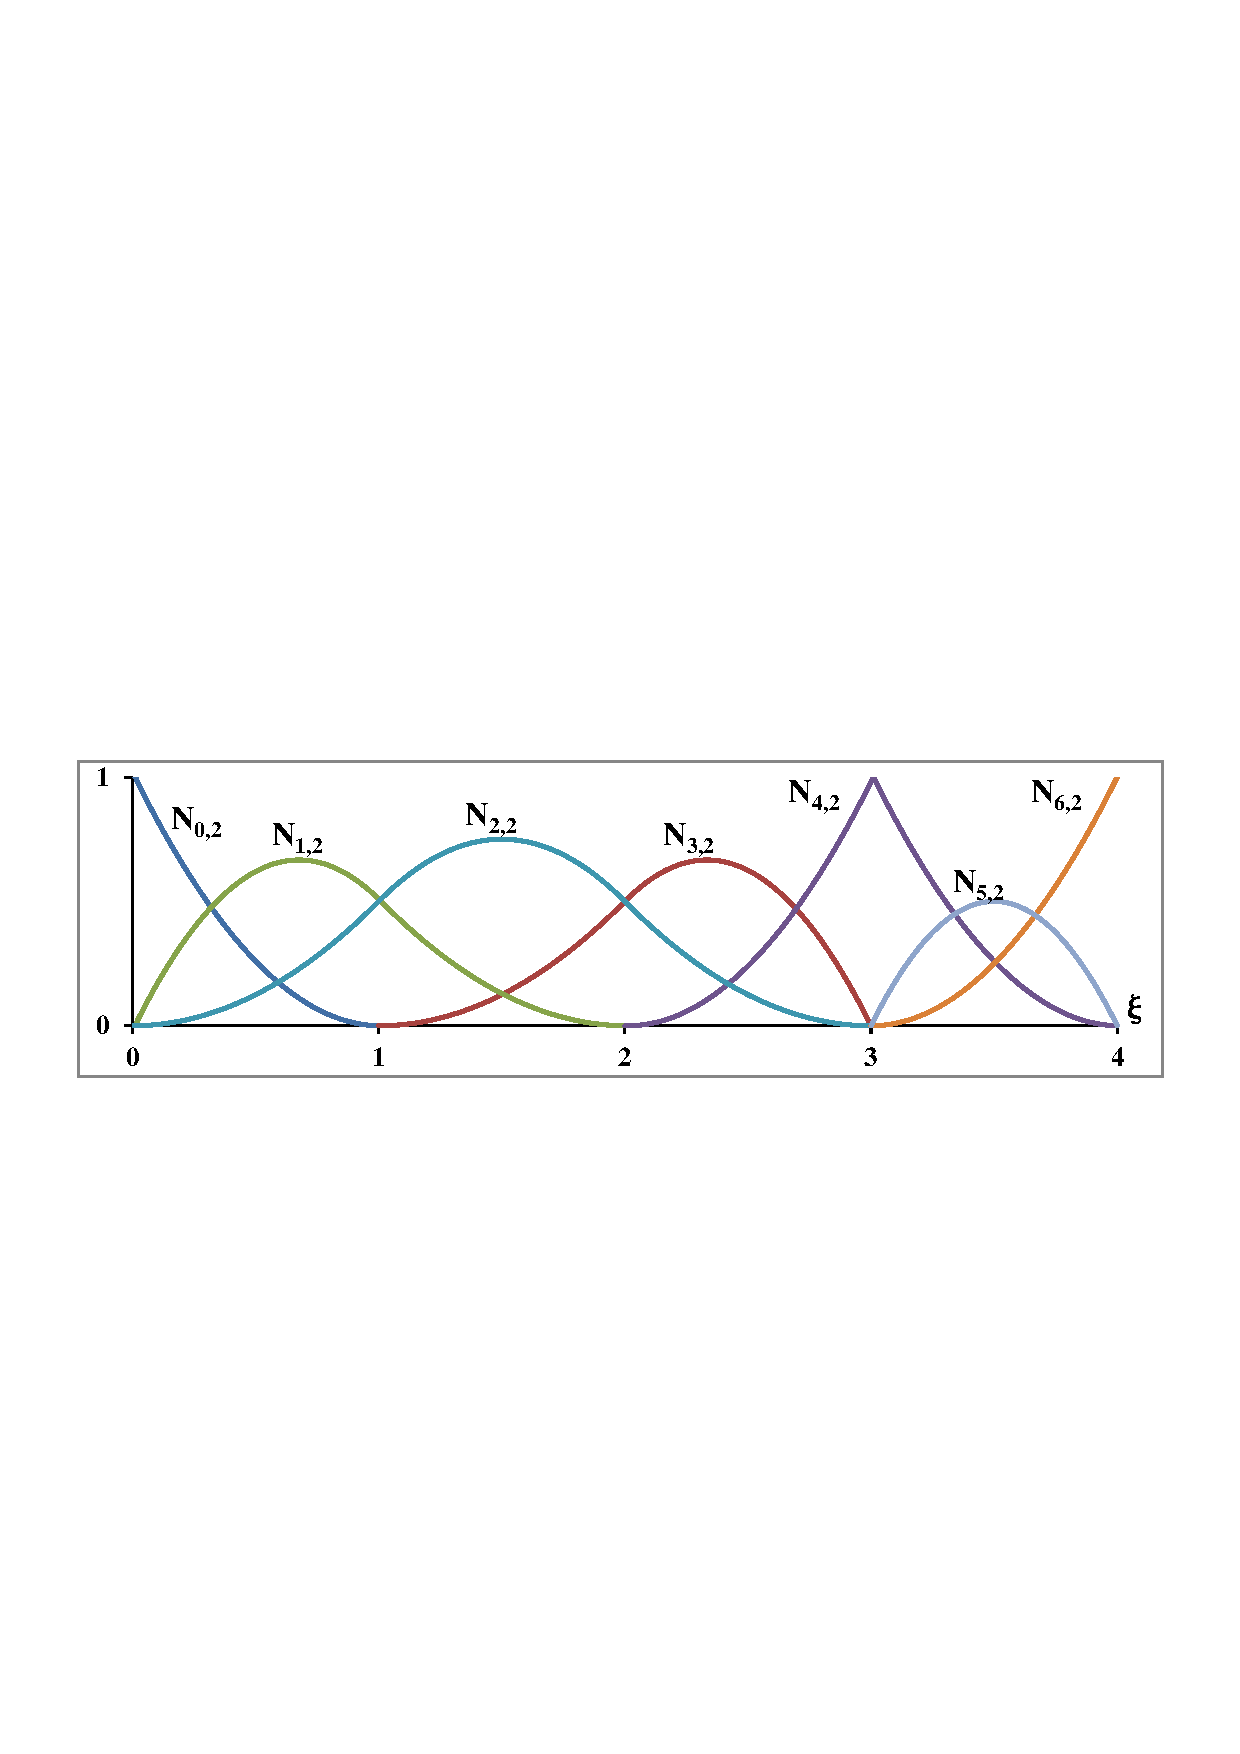
\includegraphics[scale=0.7,trim=1.5cm 11.5cm 1.5cm 13cm, clip=true]{Imagens/Cap3/bspline_funcoes.pdf}	
	\caption{\textit{B-Splines quadráticas}}
	\label{fig:bspline_funcoes}
\end{figure}

As principais propriedades das funções \textit{B-Splines} são:

\begin{itemize}
	\item \textbf{Partição da Unidade}: $\sum_{i=0}^{n}\Nb_{i,p}(\xsi)=1 $;
	\item \textbf{Positividade}: Todas as funções base são positivas, ou seja, $\Nb_{i,p}\geq0$, $\forall\xsi$;
	\item \textbf{Suavidade}: função de ordem $p$ é, em geral, $p-1$ vezes continua no contorno das células;
	\item \textbf{Suporte Compacto}: O suporte de cada $\Nb_{i,p}$ está contido no intervalo $\left[\xsi_i,\xsi_{i+p+1}\right]$, ou seja, em cada célula, apenas $p+1$ funções são não nulas. % Deve-se notar no entanto que, ao se extenderem por vários elementos, o suporte é menos compacto do que para bases formadas por polinômios de lagrange definidos em elementos finitos.
\end{itemize}

A derivada de uma função de forma \textit{B-Spline} pode ser calculada recursivamente em termos de funções base de ordem menor. Considerando uma função de ordem $p$ e vetor de \textit{knots} $\Xsi$, a derivada da i-ésima função de forma pode ser escrita como:

\begin{align}
\frac{\deriv}{\deriv \xsi} \Nb_{i,p}(\xsi) = \frac{p}{\xsi_{i+p} - \xsi_{i}}\Nb_{i,p-1}(\xsi) - \frac{p}{\xsi_{i+p+1} - \xsi_{i+1}}\Nb_{i+1,p-1}(\xsi).
\end{align}

Essa expressão pode ser generalizada para derivadas de ordem superior através de:

\begin{align}
	\frac{\deriv^{k}}{\deriv \xsi^{k}} \Nb_{i,p}(\xsi) = \frac{p!}{\left(p-k\right)!} \sum_{j=0}^{k}{\alpha_{k,j}\Nb_{i+j,p-k}(\xsi)},
\end{align}

sendo $k$ a k-ésima derivada da função $\Nb_{i,p}(\xsi)$ e:

\begin{align}
	\alpha_{0,0} = 1,
\end{align}
\begin{align}
	\alpha_{k,0} = \frac{\alpha_{k-1,0}}{\xsi_{i+p-k+1}-\xsi_{i}},
\end{align}
\begin{align}
	\alpha_{k,j} = \frac{\alpha_{k-1,j}-\alpha_{k-1,j-1}}{\xsi_{i+p+j-k+1}-\xsi_{i+j}} \ \ j=1,...,k-1,
\end{align}
\begin{align}
	\alpha_{k,k} = \frac{-\alpha_{k-1,k-1}}{\xsi_{i+p+1}-\xsi_{i+k}}.
\end{align}

Algoritmos eficientes para a determinação das funções de forma \textit{B-Splines} e de suas derivadas podem ser encontradas em \citeonline{PiegT:1996}.

\subsection{Geometrias \textit{B-Splines}}

Uma curva \textit{B-Spline} é construída a partir da combinação linear entre funções base e um conjunto de pontos de controle. Considerando um conjunto de $n+1$ funções base $\Nb_{i,p}$ e respectivos pontos de controle $\CP_i$ $\in \nrealspace$ com $i = 0,1,...,n$,
uma curva polinomial por partes \textit{B-Spline} univariada é definida como:

\begin{align}
\mathbf{C} =\pos\left(\xsi\right) = \sum_{i=0}^{n}\Nb_{i,p}(\xsi)\CP_i,
\end{align}

\noindent com $y_1$, $y_2$ e $y_3$ as componentes do vetor de coordenadas físicas $\pos$. Utilizando as funções \textit{B-Splines} apresentadas na Fig.\ref{fig:bspline_funcoes} e uma malha de $n+1$ pontos de controle, obtém-se a curva apresentada na Fig.\ref{fig:bspline_malhaPC}. Na Fig.\ref{fig:bspline_curva} pode-se observar as células físicas equivalentes a essa combinação.

\begin{figure}[!htb]
	\centering	
	\subfloat[Malha de pontos de controle\label{fig:bspline_malhaPC}]{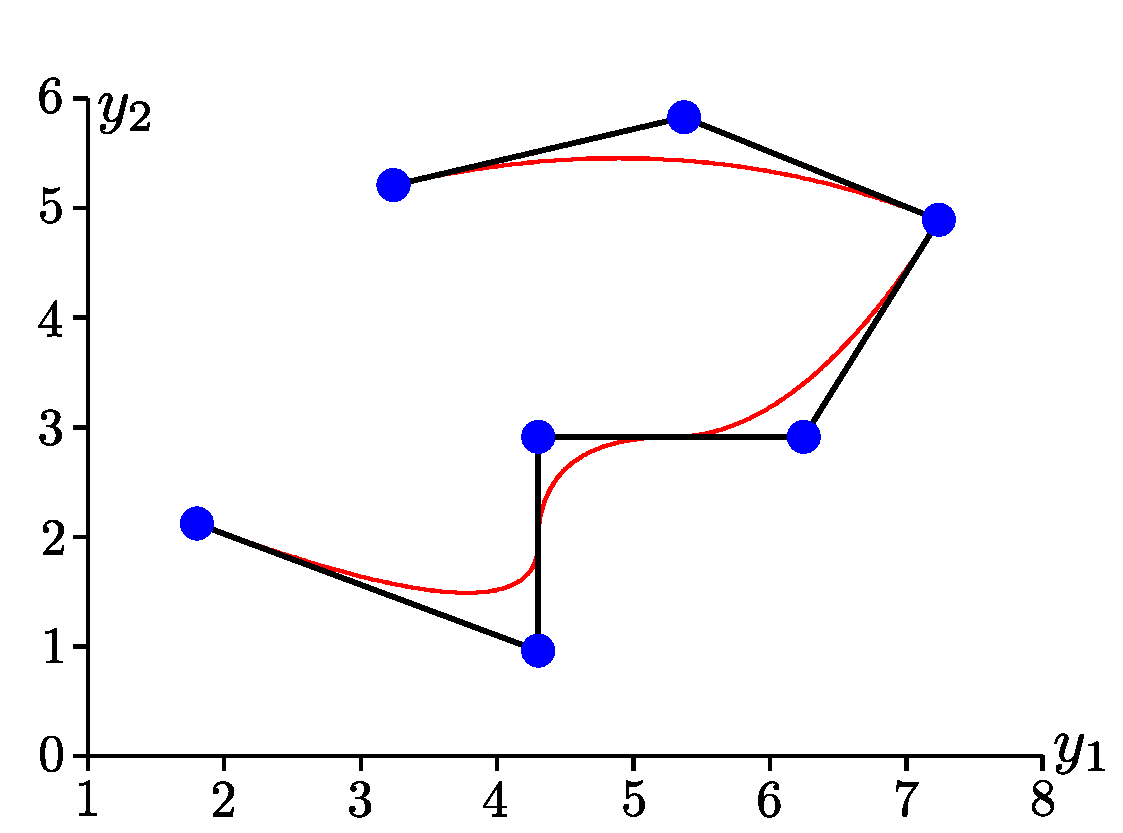
\includegraphics[scale=0.4,trim=0cm 0.0cm 0cm 0cm, clip=true]{Imagens/Cap3/bspline_malhaPC.pdf}} \ \ 
	\subfloat[Curva \textit{B-spline} e representação física das células \label{fig:bspline_curva}]{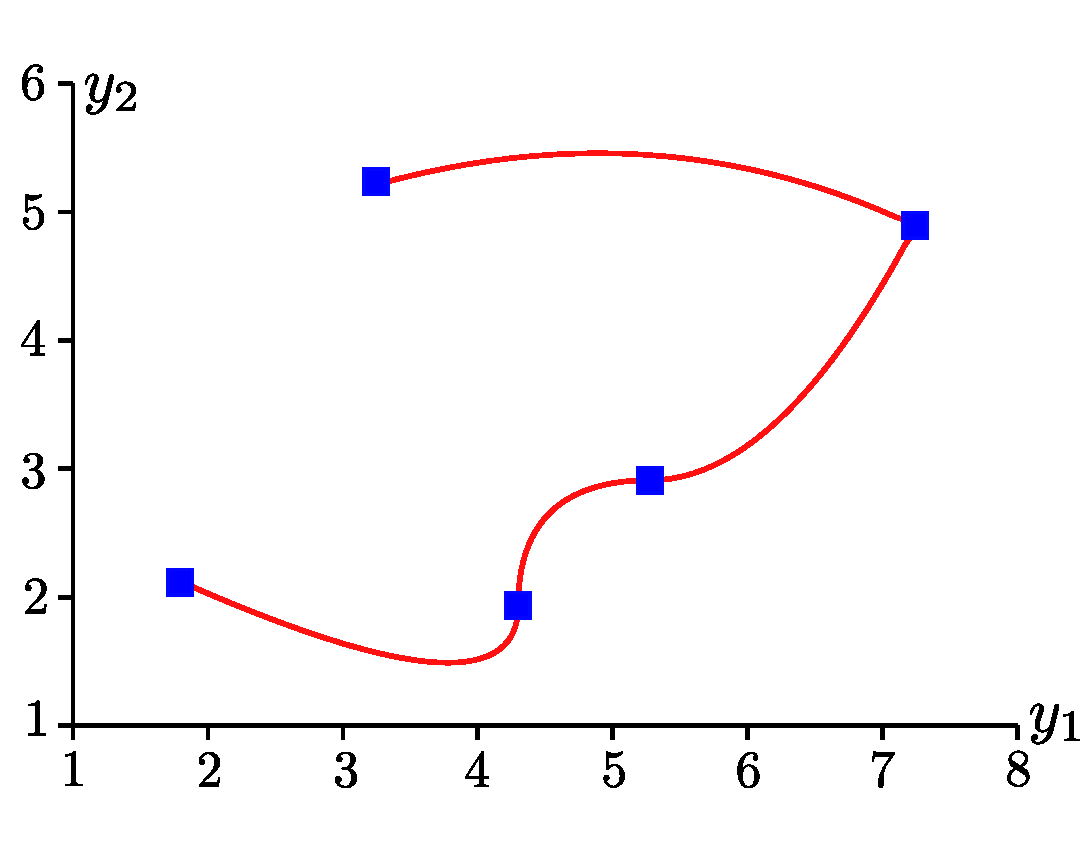
\includegraphics[scale=0.4,trim=0cm 0.7cm 0cm 0cm, clip=true]{Imagens/Cap3/bspline_curva.pdf}}
	\caption{Curva \textit{B-Spline}}
\end{figure}

A partir da Fig.\ref{fig:bspline_malhaPC} pode-se constatar que a curva \textit{B-Spline} interpola o primeiro e o último ponto de controle, que é uma característica das curvas construídas com funções descritas a partir de vetores de \textit{knots} abertos. Adicionalmente nota-se que, devido à multiplicidade do \textit{knot} de coordenada paramétrica $\xsi=3$, existe um ponto de controle intermediário também interpolando a curva. 
Coordenadas paramétricas com multiplicidade maior ou igual ao grau polinomial $p$ resultam, por definição, em interpolação dos pontos de controle associados.
Além disso, a curva possui continuidade $C^{p-1} = C^{1}$ em todos os lugares, exceto em $\xsi = 3$, onde equivale a $C^{p-2} = C^{0}$, que trata-se de uma propriedade herdada das funções base.

Conforme observado nas figuras: Fig.\ref{fig:bspline_malhaPC} e Fig. \ref{fig:bspline_curva}, muitas das características de curvas \textit{B-Splines} são consequências das propriedades das funções \textit{B-splines}. Outra importante propriedade dessas curvas é a Transformação Afim, que significa que uma transformação afim de uma curva B-spline é obtida aplicando a transformação diretamente aos pontos de controle. Além disso, devido ao suporte compacto das funções base, as curvas \textit{B-Splines} possuem característica denominada de \textit{localidade}, que significa que, movendo-se um ponto de controle, afeta-se não mais do que $p+1$ células na curva. Outras propriedades matemáticas das curvas \textit{B-Splines} podem ser consultadas em detalhes em \citeonline{PiegT:1996}.

Uma superfície \textit{B-spline} é obtida analogamente à curva \textit{B-spline}. Dado uma rede de pontos de controle $\CP_{i,j}$ $\in \nrealspace$ com $i = 0,1,...,n$ e $j = 0,1,..., m$, e vetores de \textit{knots} $\Xsi = \left[\xsi_{0},\xsi_{1},...,\xsi_{p+n+1}\right]$, $\mathcal{H} = \left[\eta_{0},\eta_{1},...,\eta_{q+m+1}\right]$, a superfície é obtida através do produto tensorial entre $(n+1)$ funções univariadas $\Nb_{i,p}$ e $(m+1)$ funções univariadas $\Mb_{j,q}$ da seguinte forma:

\begin{align}
\mathbf{S} = \pos\left(\xsi,\eta\right)  = \sum_{i=0}^{n}\sum_{j=0}^{m}\Nb_{i,p}(\xsi)\Mb_{j,q}(\eta)\CP_{i,j},
\end{align}

\noindent onde $q$ representa o grau das $m+1$ funções na direção paramétrica $\eta$. 
Muitas das propriedades das superfícies \textit{B-Splines} são resultado da natureza do produto tensorial que as geram. A base de funções apresenta propriedade de positividade e formam uma partição de unidade, de forma que: $\forall(\xsi,\eta)$ $\in \left[\xsi_{0},\xsi_{1},...,\xsi_{p+n+1}\right] \times  \left[\eta_{0},\eta_{1},...,\eta_{q+m+1}\right]$:

\begin{align}
 \sum_{i=0}^{n}\sum_{j=0}^{m}\Nb_{i,p}(\xsi)\Mb_{j,q}(\eta) = \left(\sum_{i=0}^{n} \Nb_{i,p}(\xsi)\right) \left(\sum_{j=0}^{m} \Mb_{j,q}(\eta)\right) = 1.
\end{align}

O suporte, por exemplo, de uma função bivariada $\hat{\Nb}_{i,j:p,q}\left(\xsi,\eta\right) = \Nb_{i,p}(\xsi)\Mb_{j,q}(\eta)$ é equivalente à: $\left[\xsi_{i},\xsi_{i+p+1}\right]\times\left[\eta_{j},\eta_{j+q+1}\right]$.

Por fim, um sólido \textit{B-Spline} é obtido através do produto tensorial entre funções univariadas $\Nb_{i,p}$, $\Mb_{j,q}$, $\Lb_{k,r}$, construídas sobre os vetores de \textit{knots} $\Xsi = \left[\xsi_{0},\xsi_{1},...,\xsi_{p+n+1}\right]$, $\mathcal{H} = \left[\eta_{0},\eta_{1},...,\eta_{q+m+1}\right]$ e $\mathcal{Z} = \left[\zeta_{0},\zeta_{1},...,\zeta_{r+l+1}\right]$ respectivamente, e um conjunto de pontos de controle  $\CP_{i,j,k}$ $\in \nrealspace$ com $i = 0,1,...,n$, $j = 0,1,..., m$, $k = 0,1,..., l$, da seguinte forma:

\begin{align}
\mathbf{T} = \pos\left(\xsi,\eta,\zeta\right)  = \sum_{i=0}^{n}\sum_{j=0}^{m}\sum_{k=0}^{l}\Nb_{i,p}(\xsi)\Mb_{j,q}(\eta)\Lb_{k,r}(\zeta)\CP_{i,j,k},
\end{align}

\noindent na qual $r$ representa o grau das $l+1$ funções base na direção paramétrica $\zeta$. As propriedades de um sólido \textit{B-Spline}, correspondem às generalizações trivariadas das propriedades das superfícies \textit{B-Spline}. Além disso, o suporte de uma função trivariada $\hat{\Nb}_{i,j,k:p,q,r}\left(\xsi,\eta,\zeta\right) = \Nb_{i,p}(\xsi)\Mb_{j,q}(\eta)\Lb_{k,r}(\zeta)$ está contido no intervalo $\left[\xsi_{i},\xsi_{i+p+1}\right]\times\left[\eta_{j},\eta_{j+q+1}\right]\times\left[\zeta_{k},\zeta_{k+r+1}\right]$.


\subsection{Refinamento}

Um dos aspectos mais relevantes das \textit{B-splines} é a flexibilidade na forma de enriquecimento da base, permitindo aprimorar sua representação sem alterar a geometria subjacente nem sua parametrização. Dentre os principais procedimentos utilizados, destacam-se: a inserção de \textit{knots} (ou refinamento $h$), que consiste na subdivisão da malha; a elevação de grau (ou refinamento $p$), que aumenta a ordem polinomial das funções base; o refinamento $k$, que promove simultaneamente um aumento da ordem e da continuidade entre células; e, por fim, o refinamento $hpk$, que combina de forma coordenada as três estratégias anteriores, oferecendo maior controle e eficiência na representação da geometria e na solução numérica de problemas.

Neste trabalho, será adotado na geração das geometrias o refinamento $h$, baseado na inserção de \textit{knots}. Por essa razão, somente essa estratégia será abordada ao longo desse texto.

O enriquecimento das funções base utilizando a inserção de \textit{knots} é realizado sem que se altere uma curva geometricamente ou parametricamente. Para essa finalidade, considerando o vetor de \textit{knots} $\Xsi = [\xsi_0,\xsi_1, ..., \xsi_{n+p+1}]$, será introduzido o conceito de vetor de \textit{knots} estendido, o qual compreende em: $\bar{\Xsi} = [\bar{\xsi}_0 = \xsi_0,\bar{\xsi}_1, ..., \bar{\xsi}_{n+m+p+1}= \xsi_{n+p+1}]$. As $(n+m+1)$ novas funções de base \textit{B-Splines} são determinadas através da Eq. \ref{eq:bsplines_0} e Eq. \ref{eq:bsplines_n}, aplicando-as ao vetor de \textit{knots} $\bar{\Xsi}$. Os $(n+m+1)$ novos pontos de controle  $\bar{\mathcal{B}} = [\bar{\CP}_0,\bar{\CP}_1,..., \bar{\CP}_{n+m}]^{T}$ são obtidos através da combinação linear dos $(n+1)$ pontos de controle originais, $\mathcal{B} = [\CP_0,\CP_1,..., \CP_{n}]^{T}$, por:


\begin{align}
	\bar{\mathcal{B}} = \mathbf{T}^{p}\mathcal{B},
\end{align}

\noindent, com:

\begin{align}
	\mathbf{T}_{ij}^{0} = \begin{cases} 1 &\mbox{se } \bar{\xsi}_i \in \left[\xsi_j,\xsi_{j+1}\right) \\
		0 & \mbox{caso contrário } \end{cases}, 
\end{align}

\begin{align}
	\mathbf{T}_{ij}^{q+1} = \frac{\bar{\xsi}_{i+q}-\xsi_j}{\xsi_{j+q}-\xsi_j}\mathbf{T}_{ij}^{q} + \frac{\xsi_{j+q+1}-\bar{\xsi}_{i+q}}{\xsi_{j+q+1}-\xsi_{j+1}}\mathbf{T}_{ij+1}^{q} \ \text{com} \ q=0,1,2,...,p-1,
\end{align}

\noindent sendo $i=0,1,...,(n+m)$ e $j=0,1,...,n$.

Considerando uma curva quadrática \textit{B-spline} construída sobre um vetor de \textit{knots} aberto $\Xsi=[0,0,0,1,1,1]$ apresentada na Fig. \ref{fig:bspline_pc_ai} juntamente com sua rede de pontos de controle. Essa curva, possui apenas uma célula no espaço físico, conforme pode ser observado na Fig. \ref{fig:bspline_curva_ai}, e $3$ funções base no espaço paramétrico (Fig. \ref{fig:bspline_base_ai}). Ao realizar-se a inserção de um \textit{knot}, $\xsi=1/2$, o vetor de \textit{knots} estendido fica definido como: $\bar{\Xsi}=[0,0,0,1/2,1,1,1]$. Aplicando-se as Eq. \ref{eq:bsplines_0} e Eq. \ref{eq:bsplines_n} à esse vetor de coordenadas paramétricas, obtém-se as $4$ funções base apresentadas na Fig.\ref{fig:bspline_base_di} definidas sobre 2 células do espaço paramétrico. Após o emprego do refinamento $h$, a geometria da curva é preservada. No entanto, como ilustrado na Fig. \ref{fig:bspline_curva_di}, uma nova célula física é inserida, além de que, de acordo com a Fig. \ref{fig:bspline_pc_di}, a malha de pontos de controle é modificada, com o acréscimo de um novo ponto e o reajuste de suas posições.


\begin{figure}[!t]
	\centering
	\subfloat[\label{fig:bspline_pc_ai}Curva original e pontos de pontrole]{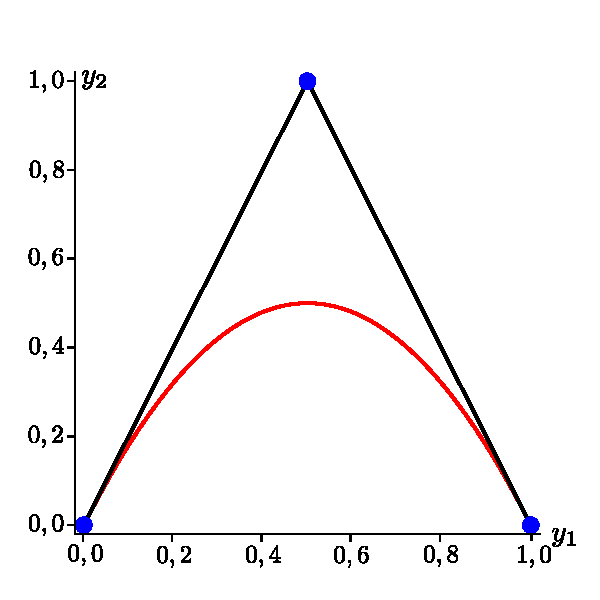
\includegraphics[scale=0.7,trim=0cm 0cm 0cm 1cm, clip=true]{Imagens/Cap3/bspline_pc_ai.pdf}} 
	\subfloat[\label{fig:bspline_pc_di}Curva refinada e pontos de controle]{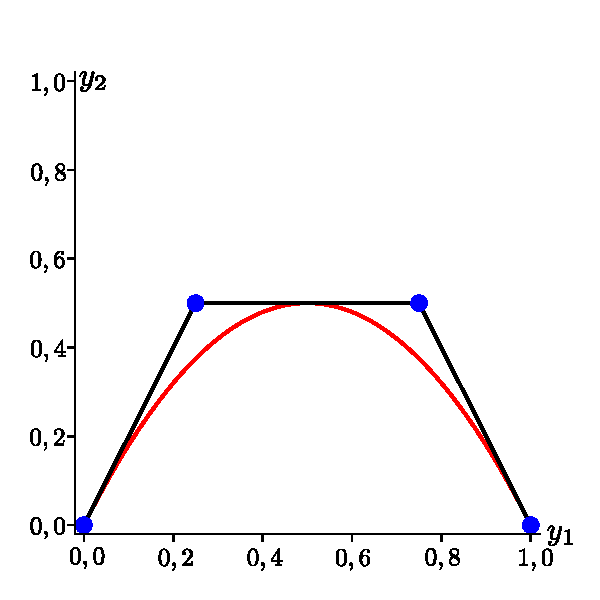
\includegraphics[scale=0.7,trim=0cm 0cm 0cm 1cm, clip=true]{Imagens/Cap3/bspline_pc_di.pdf}} \\ 
	\subfloat[\label{fig:bspline_curva_ai}Célula curva original]{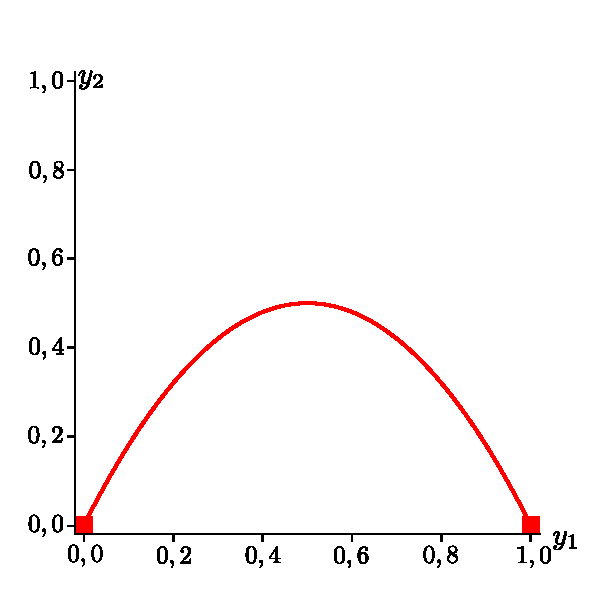
\includegraphics[scale=0.7,trim=0cm 0cm 0cm 1cm, clip=true]{Imagens/Cap3/bspline_curva_ai.pdf}} 
	\subfloat[\label{fig:bspline_curva_di}Células curva refinada]{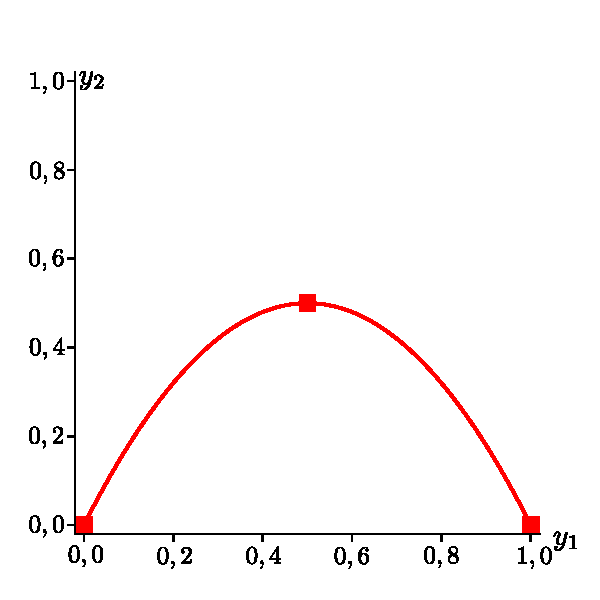
\includegraphics[scale=0.7,trim=0cm 0cm 0cm 1cm, clip=true]{Imagens/Cap3/bspline_curva_di.pdf}} \\ 
	\subfloat[\label{fig:bspline_base_ai}Funções base originais]{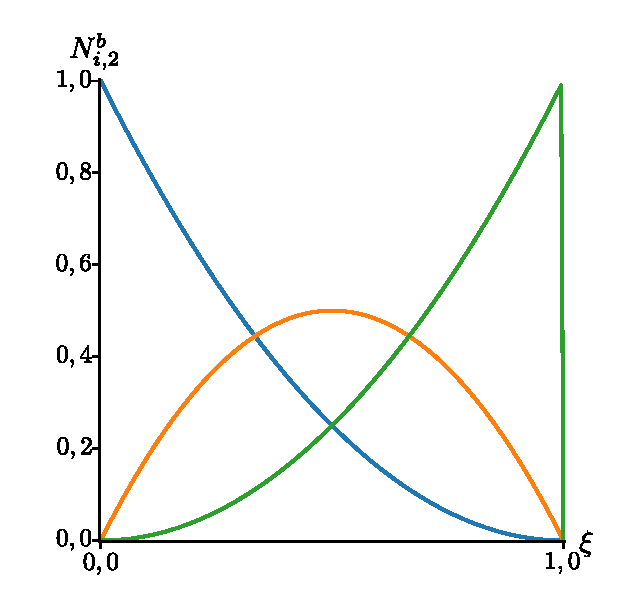
\includegraphics[scale=0.7,trim=0cm 0cm 0cm 0.5cm, clip=true]{Imagens/Cap3/bspline_base_ai.pdf}} 
	\subfloat[\label{fig:bspline_base_di}Funções base após refinamento $h$ refinada]{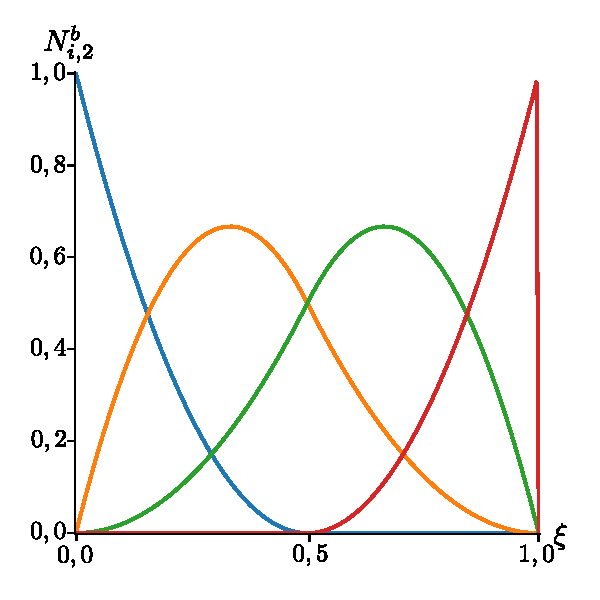
\includegraphics[scale=0.7,trim=0cm 0cm 0cm 0.4cm, clip=true]{Imagens/Cap3/bspline_base_di.pdf}} 
	\caption{Refinamento $h$ para um curva \textit{B-Spline}}
	\label{fig:bspline_insercaoKnots}
\end{figure}

Para fins práticos, o processo de refinamento consiste na inserção consecutiva de coordenadas paramétricas ao vetor de \textit(knots) até que se alcance a discretização desejada. Um algoritmo mais eficiente para realizar esse procedimento de refinamento pode ser encontrado em \citeonline{PiegT:1996}. Esse procedimento pode ser aplicado analogamente à superfícies e sólidos, aplicando-se a inserção de \textit{knots} nas direções paramétricas desejadas.


\section{NURBS}

Uma geometria NURBS no $\nrealspace$ pode ser entendida, do ponto de vista geométrico, como a transformação projetiva de uma geometria \textit{B-Spline} no $\realspace^{\nsd+1}$. Nesse contexto, geometrias cônicas podem ser construídas exatamente através de curvas quadráticas por partes. Na Fig. \ref{fig:NURBS_curva_transProj}, apresenta-se uma curva NURBS $\mathbf{C}\left(\xsi\right)$ no $\realspace^{2}$ , que representa de forma exata uma circunferência, a qual foi obtida a partir da transformação projetiva de uma curva quadrática por partes \textit{B-Spline} ($\mathbf{C}^{w}\left(\xsi\right)$) no  $\realspace^{3}$. A transformação é realizada através da projeção em um plano $y_3 = 1$ de cada ponto da curva projetiva ($\mathbf{C}^{w}\left(\xsi\right)$) através de um raio que passa pela origem.

\begin{figure}[!htb]
	\centering	
	\subfloat[Projeção transformativa malha de pontos de controle\label{fig:NURBS_PC_transProj}]{\includegraphics[scale=0.4,trim=0cm 0.0cm 0cm 0cm, clip=true]{Imagens/Cap3/NURBS_PC_projetiva.pdf}} \ \ 
	\subfloat[Projeção transformativa \textit{B-Spline} \label{fig:NURBS_curva_transProj}]{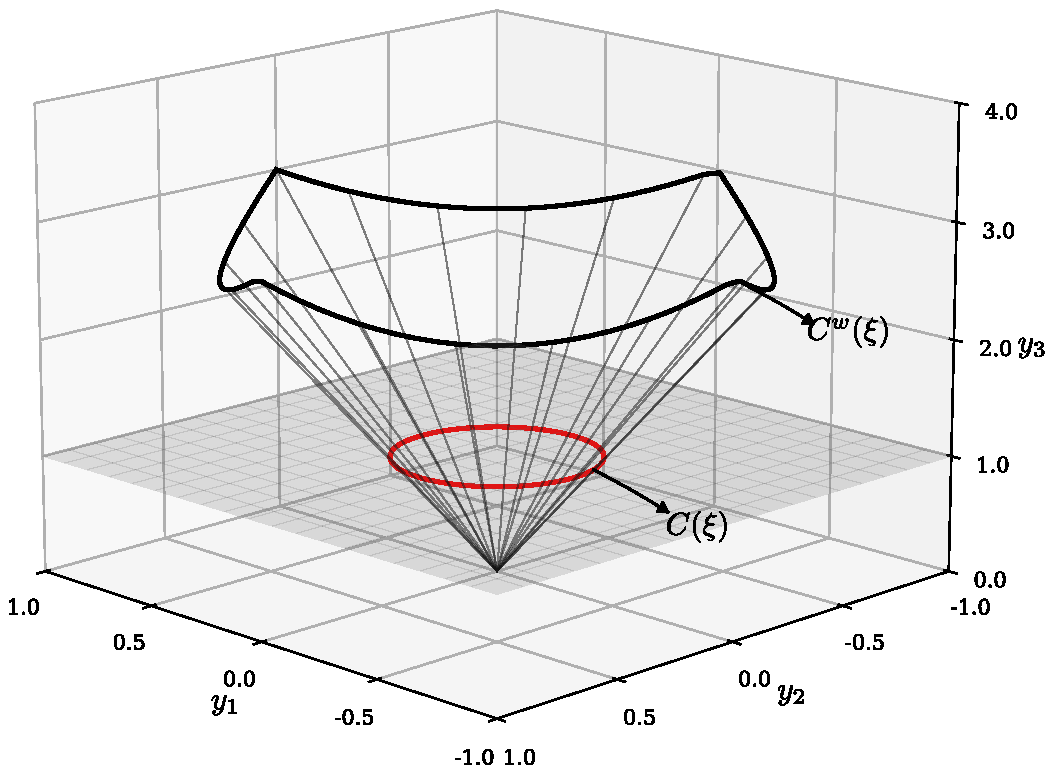
\includegraphics[scale=0.4,trim=0cm 0.0cm 0cm 0cm, clip=true]{Imagens/Cap3/NURBS_curva_projetiva.pdf}}
	\caption{Projeção transformativa de entidade \textit{B-Spline}}
\end{figure}

O mesmo procedimento de transformação pode ser realizado para obtenção dos pontos de controle NURBS (Fig. \ref{fig:NURBS_PC_transProj}) a partir de pontos de controle projetivos ($\mathbf{B_i}^w$), usando a seguinte relação:

\begin{align}
	\left(\CP_i\right)_j = \left(\CP^w_i\right)_j/w_i, \ \ j=1,...,\nsd ,
\end{align}

\begin{align}
	w_i =   \left(\CP^w_i\right)_{\nsd+1},
\end{align}

\noindent com $\left(\CP_i\right)_j$ o j-ésimo componente do vetor $\CP_i$ e $w_i$ refere-se ao i-ésimo peso, que consiste na coordenada $y_3$ dos pontos de controle projetivos para o exemplo citado.

Para a aplicação dessa mesma transformação para cada ponto da curva, será utilizado um conceito de função peso, dada por:

\begin{align}
	W(\xsi) = \sum_{\hat{i}=0}^{n}\Nb_{\hat{i},p}(\xsi)w_{\hat{i}},
\end{align}

e a curva NURBS pode ser definida como:

\begin{align}
	\left(\mathbf{C}(\xsi)\right)_j = \left(\mathbf{C}^w(\xsi)\right)_j/W(\xsi), \ \ j = 1,...,\nsd.
\end{align}

Tanto $\mathbf{C}^w$ como $W(\xsi)$ são funções polinomiais por partes, dessa forma, $\mathbf{C}(\xsi)$ é uma função racional por partes.

\subsection{Funções base NURBS e suas derivadas}

Matematicamente, uma função NURBS é obtida pela racionalização de uma função \textit{B-Spline}. A racionalização dessa função ocorre através da razão entre dois polinômios. Uma função racional NURBS $\left(\fNURBS\right)$ é construída através da seguinte expressão:

\begin{align}
\fNURBS_{i,p}(\xsi) = \frac{\Nb_{i,p}(\xsi)w_i}{\sum_{\hat{i}=0}^{n}\Nb_{\hat{i},p}(\xsi)w_{\hat{i}}}.  \label{eq:NURBS_function}
\end{align}

\noindent com $w_{i}$ e $w_{\hat{i}}$ $\in \realspace$, sendo $i = \hat{i} =  0, 1, ... , n$.

A derivada de uma função $\fNURBS_{i,p}$ é obtida aplicando simplesmente a regra do quociente à expressão da Eq. \ref{eq:NURBS_function}:

\begin{align}
	\frac{\deriv}{\deriv \xsi} \fNURBS_{i,p}(\xsi) = w_{i} \frac{W\left(\xsi\right)\Nbl\left(\xsi\right) - W^{'}\left(\xsi\right)\Nb_{i,p}\left(\xsi\right)}{\left(W\left(\xsi\right)\right)^2},
\end{align}

\noindent com:

\begin{align}
	\Nbl\left(\xsi\right) \equiv \frac{\deriv}{\deriv \xsi} \Nb_{i,p}\left(\xsi\right),
\end{align}

\noindent e:

\begin{align}
	W^{'}\left(\xsi\right) = \sum_{\hat{i}=0}^{n} \Nblc \left(\xsi\right) w_{\hat{i}}.
\end{align}

A $k$-ésima derivada de $\fNURBS_{i,p}$ é obtida em termos de derivadas de menores ordem, através da seguinte expressão:

\begin{align}
\frac{\deriv^{k}}{\deriv \xsi^{k}} \fNURBS_{i,p}(\xsi) = \frac{A_{i}^{\left(k\right)} \left(\xsi\right) - \sum_{j=1}^{k} \binom{k}{j} W^{\left(j\right)} \left(\xsi\right) \frac{\deriv^{(k-j)}}{\deriv \xsi^{(k-j)}}\fNURBS_{i,p} \left(\xsi\right)}{W\left(\xsi\right)}
\end{align}

\noindent com:

\begin{align}
\binom{k}{j} = \frac{k!}{j!\left(k-j\right)!} ,
\end{align}

\begin{align}
	W^{\left(j\right)}\left(\xsi\right) = \frac{\deriv^{j}}{\deriv \xsi^{j}} W \left(\xsi\right) ,
\end{align}

\noindent e:

\begin{align}
 A_{i}^{\left(k\right)} \left(\xsi\right)  = w_i \frac{\deriv^k}{\deriv\xsi^k}\Nb_{i,p} \left(\xsi\right)\text{sem soma em $i$}.
\end{align}

\subsection{Geometria NURBS}

Uma curva NURBS é obtida através da combinação linear entre as funções base NURBS e um conjunto de pontos de controle, conforme expresso pela equação abaixo: 

\begin{align}
\mathbf{C} = \pos\left(\xsi\right) = \sum_{i=0}^{n}\fNURBS_{i,p}(\xsi)\CP_i, \label{eq:curveNURBS}
\end{align}

\noindent cujos pontos de controle e pesos são escolhidos criteriosamente de forma a obter-se a geometria desejada.

Analogamente uma superfície NURBS é obtida através das seguintes relações:

\begin{align}
\fNURBS_{i,j:p,q}(\xsi,\eta) = \frac{\Nb_{i,p}(\xsi)\Mb_{j,q}(\eta)w_{i,j}}{\sum_{\hat{i}=0}^{n}\sum_{\hat{j}=0}^{m}\Nb_{\hat{i},p}(\xsi)\Mb_{\hat{j},q}(\eta)w_{\hat{i},\hat{j}}},
\end{align}

\begin{align}
\mathbf{S} = \pos\left(\xsi,\eta\right) = \sum_{i=0}^{n}\sum_{j=0}^{m}\fNURBS_{i,j:p,q}(\xsi,\eta)\CP_{i,j}, \label{eq:surfaceNURBS}
\end{align}

\noindent com $w_{i,j}$ e $w_{\hat{i},\hat{j}}$ $\in \realspace$, sendo $i = \hat{i} =  0, 1, ... , n$ e  $j = \hat{j} =  0, 1, ... , m$ , correspondem aos pesos relativos às funções $\Nb_{i,p}\left(\xsi\right)\Mb_{j,q}\left(\eta\right)$ e $\Nb_{\hat{i},p}\left(\xsi\right)\Mb_{\hat{j},q}\left(\eta\right)$ respectivamente. Por fim, um sólido NURBS é obtido por:

\begin{align}
\fNURBS_{i,j,k:p,q,r}(\xsi,\eta,\zeta) = \frac{\Nb_{i,p}(\xsi)\Mb_{j,q}(\eta)\Lb_{k,r}(\zeta)w_{i,j,k}}
{\sum_{\hat{i}=0}^{n}\sum_{\hat{j}=0}^{m}\sum_{\hat{k}=0}^{l}\Nb_{\hat{i},p}(\xsi)\Mb_{\hat{j},q}(\eta)\Lb_{\hat{k},r}(\zeta)w_{\hat{i},\hat{j},\hat{k}}},
\end{align}

\begin{align}
\mathbf{T} = \pos\left(\xsi,\eta,\zeta\right) = \sum_{i=0}^{n}\sum_{j=0}^{m}\sum_{k=0}^{l}\fNURBS_{i,j,k:p,q,r}(\xsi,\eta,\zeta)\CP_{i,j,k}, \label{eq:solidNURBS}
\end{align}

\noindent onde $w_{i,j,k}$ e $w_{\hat{i},\hat{j},\hat{k}}$ $\in \realspace$, sendo $i = \hat{i} =  0, 1, ... , n$, $j = \hat{j} =  0, 1, ... , m$ e $k = \hat{k} =  0, 1, ... , l$, correspondem aos pesos relativos às funções $\Nb_{i,p}\left(\xsi\right)\Mb_{j,q}\left(\eta\right)\Lb_{k,r}\left(\zeta\right)$ e $\Nb_{\hat{i},p}\left(\xsi\right)\Mb_{\hat{j},q}\left(\eta\right)\Lb_{\hat{k},r}\left(\zeta\right)$, respectivamente.

\subsection{Múltiplos \textit{Patches}}

Na grande maioria das situações práticas, é necessário para descrever um domínio computacional o uso de múltiplos \textit{patches} NURBS, isto se deve ao fato que o produto tensorial do espaço paramétrico não é adequado para a representação de domínios complexos multiplamente conectados. Ademais, mesmo para domínios simples, do ponto de vista da simulação numérica, o uso de múltiplos \textit{patches} pode ser necessário em algumas circunstâncias, conforme será visto na seção de exemplos.

\citeonline{HughesCB:2005} cita que o uso de múltiplos \textit{patches} pode facilitar a análise numérica quando diferentes materiais e modelos físicos são utilizados em diferentes partes do domínio. E, além disso, em processamento paralelo, pode se tornar conveniente, do ponto de vista de estruturas de dados, não ter um único \textit{patch} entre diferentes processadores.

A utilização de múltiplos \textit{patches} implica na compatibilização da discretização na interface entre \textit{patches} adjacentes, ou seja, a parametrização e o mapeamento devem ser idênticos nesses locais. Cada ponto de controle em uma face de \textit{patches} adjacentes deve possuir um correspondente na outra face. Esses pontos iguais são tratados como um único ponto de controle dentro do sistema global resultante da análise numérica. 

Ressalta-se ainda, que na interface entre os \textit{patches}, devido a natureza interpolatória do vetores de \textit{knots} abertos, as funções base terão continuidade $C_0$, conforme pode ser observado na Fig. \ref{fig:multiplos_patches}, onde apresentam-se as funções base univariadas na interface entre dois \textit{patches}.

\begin{figure}[htb!]
	\centering 
	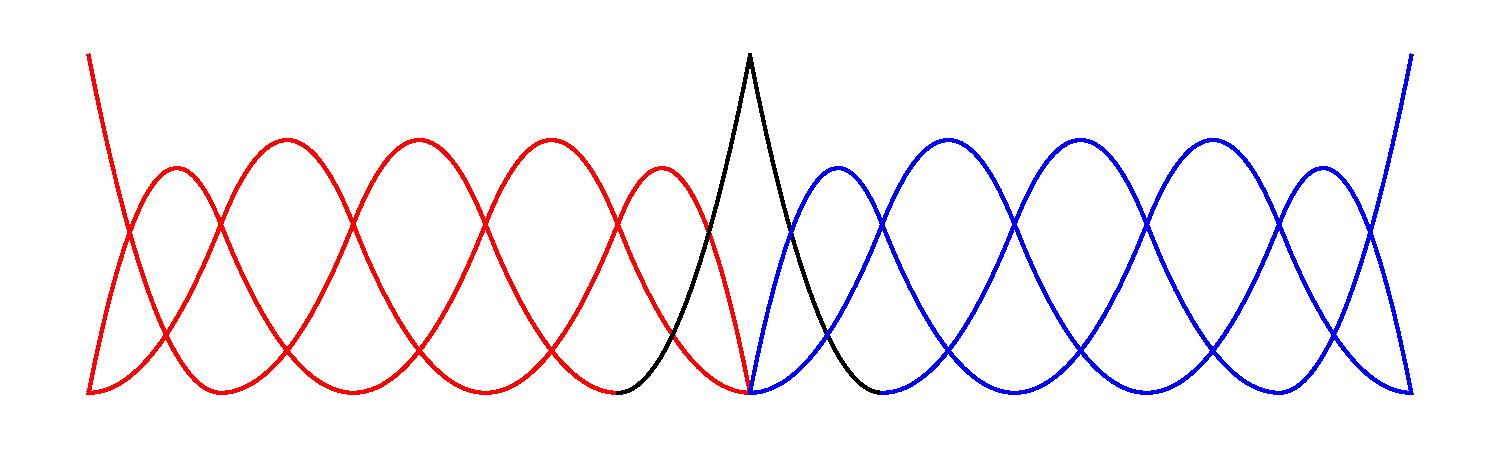
\includegraphics[scale=0.5,trim=0cm 0cm 0cm 0cm, clip=true]{Imagens/Cap3/patches.pdf}	
	\caption{Funções base univariadas na interface entre \textit{patches}}
	\label{fig:multiplos_patches}
\end{figure}


\section{Análise Isogeométrica}\label{capitulo:Cap3:IGA}


Para a aplicação da IGA no contexto da Dinâmica dos Fluidos Computacional, será utilizada como base a metodologia apresentada no Cap. \ref{capitulo:Cap2}. Nesse contexto, a aproximação da geometria, realizada no contexto do MEF pela Eq. \ref{eq:interp_geo}, será substituída pela abordagem Isogeométrica através do uso de geometrias NURBS, descritas pelas equações: Eq. \ref{eq:curveNURBS}, Eq. \ref{eq:surfaceNURBS} ou Eq. \ref{eq:solidNURBS} para os casos de curvas, superfícies ou sólidos, respectivamente.

As funções tentativa para velocidade e pressão, e as funções teste associadas à elas, apresentadas nas Eq. \eqref{eq:interp_vel} à Eq. \eqref{eq:inter_ptest} como $N$, são equivalentes à $\fNURBS_{i,p}(\xsi)$, $\fNURBS_{i,j:p,q}(\xsi,\eta)$ e $\fNURBS_{i,j,k:p,q,r}(\xsi,\eta,\zeta)$ a depender da geometria em análise.

A integração numérica nas células é realizada através da quadratura Gaussiana. Considerando o domínio paramétrico de uma célula: $\bar{\domain}^{e}$, e o domínio de integração ou parental: $\tilde{\domain}^{e}$, apresentados na Fig.\ref{fig:espacos_NURBS}, definidos respectivamente pelos vetores de coordenadas paramétricas $\coordAdimen\left(\xsi,\eta,\zeta\right)$ e $\tilde{\coordAdimen}(\tilde{\xsi},\tilde{\eta},\tilde{\zeta})$, a matriz jacobiana do mapeamento do espaço físico, com coordenadas $\pos \left(y_1,y_2,y_3\right)$,  para o espaço de quadratura, é definida por:

\begin{align}
\frac{d\pos}{d\tilde{\coordAdimen}} = \frac{d\pos}{d\coordAdimen} \frac{d\coordAdimen}{d\tilde{\coordAdimen}}, \label{eq:integ}
\end{align} 

\noindent com $\tilde{\xi}, \tilde{\eta}, \tilde{\zeta} \in [-1, 1]$.

O primeiro termo à direita da igualdade da Eq. \eqref{eq:integ} é calculado a partir das derivadas parciais da Equação: Eq. \eqref{eq:curveNURBS}, Eq. \eqref{eq:surfaceNURBS} ou Eq. \eqref{eq:solidNURBS}, a depender do tipo da geometria em questão (curva, superfície ou sólido, respectivamente).

Para a obtenção do segundo termo à direita, primeiramente é necessário definir-se a relação entre as coordenadas  do domínio paramétrico e do domínio parental. Considerando-se a célula $\bar{\domain}^{e} = [\xsi_{i},\xsi_{i+1}] \times [\eta_{j},\eta_{j+1}] \times [\zeta_{k},\zeta_{k+1}]$, pode-se calcular $\xsi,\eta, \zeta$ $\in \bar{\domain}^{e}$ a partir de $\tilde{\xsi},\tilde{\eta}, \tilde{\zeta}$ $\in \tilde{\domain}^{e}$ através das seguintes relações: 

\begin{align}
\xsi = \xsi_{i} + \left(\tilde{\xsi}+1\right) \left(\frac{\xsi_{i+1}-\xsi_{i}}{2}\right), \label{eq:derXsi}
\end{align}

\begin{align}
\eta = \eta_{i} + \left(\tilde{\eta}+1\right) \left(\frac{\eta_{i+1}-\eta_{i}}{2}\right), \label{eq:derNeta}
\end{align}

\noindent e

\begin{align}
\zeta = \zeta_{i} + \left(\tilde{\zeta}+1\right) \left(\frac{\zeta_{i+1}-\zeta_{i}}{2}\right), \label{eq:derZeta}
\end{align}

\noindent assim, $\frac{d\coordAdimen}{d\tilde{\coordAdimen}}$ é obtido derivando-se parcialmente às expressões apresentadas em: Eq. \ref{eq:derXsi}, Eq. \ref{eq:derNeta} e Eq. \ref{eq:derZeta}.


\subsection{Parâmetros de estabilização}\label{capitulo:Cap3:RepreGeo:taus2}

Para a determinação dos parâmetros de estabilização $\tau$, de acordo com o exposto na Subseção \ref{capitulo:Cap2:FormaFraca:taus}, faz-se necessário a determinação de um tensor métrico, $\matrixG$ (Eq. \ref{eq:tensor_metrico}), o qual depende da matriz jacobiana transformada, $\matrixQhat$, definida na Eq. \ref{eq:q_chap}.

Devido a diferença entre o espaço paramétrico utilizado na definição das funções de base e do espaço paramétrico de integração, definido aqui como espaço parental, a matriz $\matrixQ$ será reescrita como:

\begin{align}
	\matrixQ&=\left(\frac{\partial\pos}{\partial\tilde{\coordAdimen}}\right).
\end{align}

Para a obtenção de $\matrixQhat$, de acordo com a Eq. \ref{eq:q_chap}, define-se a matriz $\matrixD$ para análise isogeométrica, de acordo com o trabalho de \citeonline{OtoguroTT:2020}, como:

\begin{align}
	\matrixD&=\left(\frac{\partial\hat{\coordAdimen}}{\partial\tilde{\coordAdimen}}\right),
\end{align}

\noindent que representa a relação entre o espaço paramétrico de preferência, onde o comprimento efetivo da célula deve ser medido, e o espaço de integração, onde são definidos os pontos de quadratura.

O espaço paramétrico de preferência, para problemas unidimensionais, é definido para cada célula por meio de uma interpolação usando polinômios de Bernstein $B_{b}^{p}$ de ordem $p$:

\begin{align}
	\hat{\xsi} \left(\tilde{\xsi}\right) = \sum_{b=0}^{p} \hat{\xsi}_b B_{b}^{p}\left(\tilde{\xsi}\right),
\end{align}

\noindent com os pontos de controle de Bézier, $\hat{\xsi}_b$, definidos igualmente espaçados da seguinte maneira:

\begin{align}
	\hat{\xsi}_b = \frac{\Delta{\hat{\xsi}}}{p}b,
\end{align}

\noindent sendo $\Delta{\hat{\xsi}}$ o comprimento paramétrico da célula de Bézier. 

Os pontos de controle correspondentes no espaço de integração são dados por:

\begin{align}
	\tilde{\xsi}_a = \frac{\Delta{\hat{\xsi}}}{p} \sum_{b=0}^{p}b\left\{\matrixCinv\right\}_{ba},
\end{align}

\noindent com $a=0,...,p$. $\matrixC$ consiste no operador de extração de Bézier, que relaciona as funções B-spline globais às funções de Bernstein locais, cuja obtenção, nesse trabalho, é realizada de acordo com o exposto em \citeonline{BordenSEH}.

O comprimento efetivo da célula para $a = 1, ..., p$ pode ser calculado por:

\begin{align}
	\Delta{\tilde{\xsi}_a} &= \tilde{\xsi}_a - \tilde{\xsi}_{a-1} \\
		           &= \frac{\Delta{\hat{\xsi}}}{p} \sum_{b=0}^{p}b\left(\left\{\matrixCinv\right\}_{ba} - \left\{\matrixCinv\right\}_{ba-1}\right).
\end{align}


A partir disso pode-se definir o razão entre o comprimento da célula de Bézier e o comprimento efetivo da célula. Considerando um problema 1D, uma das proposta dos autores para $D$, utilizada nesse trabalho, chama-se \textit{RQD-MAX} e consiste em:


\begin{align}
	D&=\frac{\Delta\hat{\xsi}}{\min_{a=1,...,p} \Delta\tilde{\xsi_{a}}},
\end{align}

\noindent resultando em:

\begin{align}
	D&={p}\left(\min_{a=1,...,p} \sum_{b=0}^{p} b \left(\left\{\matrixCinv\right\}_{ba} - \left\{\matrixCinv\right\}_{ba-1}\right)\right)^{-1} \\
	  &={p}\max_{a=1,...,p}\left(\sum_{b=0}^{p} b \left(\left\{\matrixCinv\right\}_{ba} - \left\{\matrixCinv\right\}_{ba-1}\right)\right)^{-1}
\end{align}

Para múltiplas dimensões o coeficiente de transformação $D$ é obtido individualmente para cada uma das direções do espaço paramétrico, e os componentes da matriz de transformação $\matrixD$ são determinados como:

\begin{align}
	D_{ij} = D^{i} \delta_{ij},
\end{align}

\noindent $i,j = 1,...,n_{pd}$, sendo $n_{pd}$ a dimensão do espaço paramétrico.


\section{Verificação e aplicações}

Para aplicação da IGA em problemas da DFC utilizou-se o roteiro da implementação computacional apresentada no Alg. \ref{capitulo:Cap2:DFCComputationalCode}, levando-se em consideração as mudanças na formulação salientadas na Seção \ref{capitulo:Cap3:IGA}. Os exemplos escolhidos para a verificação do código computacional foram o escoamento sobre um cilindro, e um escoamento sobre canal com degrau, em ambas análises, fez-se uso de células 3d. Os resultados obtidos são apresentados nas subseções sequentes.

\subsection {Escoamento sobre um cilindro}

\subsubsection {Geração da malha NURBS} \label{Cap3:VerApl:Cilindro:Malha}

Para a análise do problema de escoamento sobre um cilindro utilizando-se IGA  com células 3d, por se tratar de uma geometria de simples complexidade, a malha foi desenvolvida pela própria autora. Para isso, inicialmente, com base nas dimensões bidimensionais do exemplo apresentado na Subseção \ref{capitulo:Cap2:VerApl:Cilindo}, dividiu-se o domínio físico em 12 \textit{patches}, conforme pode ser observado no esquema apresentado na Fig. \ref{fig:cilindro_IGA_patches}.

\begin{figure}[htb!]
	\centering 
	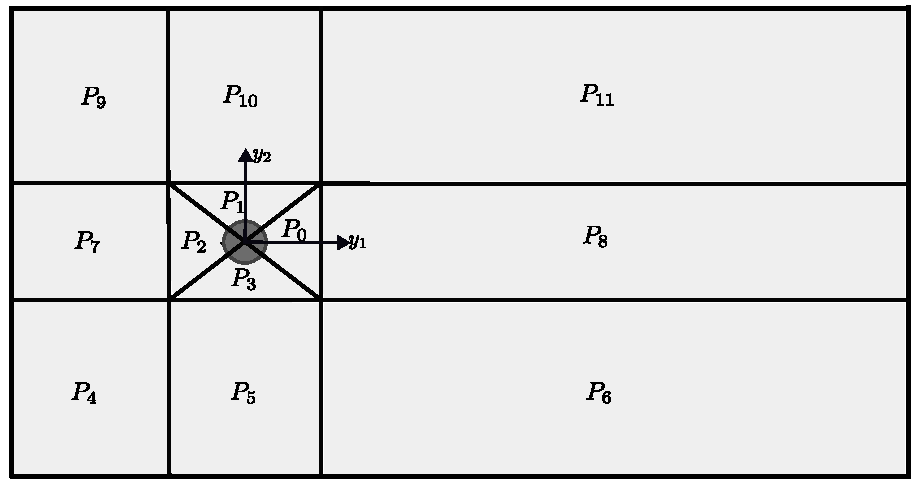
\includegraphics[scale=0.7,trim=0cm 0cm 0cm 0cm, clip=true]{Imagens/Cap3/cilindro_iga_patches.pdf}	
	\caption{Cilindro: Divisão dos \textit{Patches} }
	\label{fig:cilindro_IGA_patches}
\end{figure}

O processo de geração da malha, simplificadamente, consiste em se escolher vetores de $knots$, pontos de controle, e pesos adequados para a descrição da geometria de cada \textit{patch}, assegurando simultaneamente o refinamento necessário para a análise numérica.

Para a geração do primeiro \textit{patch}, $P_0$, o qual contém $1/4$ do cilindro em seu interior, iniciou-se pela discretização de uma circunferência definida na direção paramétrica $\xsi$. Utilizando o número mínimo de pontos de controle necessários para representar exatamente $1/4$ de circunferência, de diâmetro D, com o uso de funções quadráticas NURBS, o vetor de \textit {knots} aberto foi definido por: $\Xsi=\left[0,0,0,1,1,1\right]$, os pontos de controle como: $\CP_0=[\frac{\sqrt{2}D}{4},-\frac{\sqrt{2}D}{4},0]$, $\CP_1=[\frac{D}{\sqrt{2}},0,0]$, $\CP_2=[\frac{\sqrt{2}D}{4},\frac{\sqrt{2}D}{4},0]$, e os pesos: $w_0 = 1$, $w_1 = \frac{\sqrt{2}}{2}$ e $w_2 = 1$. A disposição dos pontos de controle e a curva resultante, podem ser observados na Fig. \ref{fig:cilindro_circ_ini}.

Na sequência realizou-se o procedimento de refinamento por inserção sucessiva de coordenadas paramétricas no vetor de \textit{knots}. O algoritmo utilizado para este procedimento pode ser encontrado em \citeonline {PiegT:1996}. Na Fig. \ref{fig:cilindro_circ_ref} apresenta-se um exemplo dos pontos de controle resultantes após a inserção das coordenadas paramétricas $1/4, 1/2 \ \text{e} \ 3/4$. Essa inserção resultará em três novas células físicas. A quantidade de coordenadas paramétricas a ser inserida depende da discretização requerida à analise numérica.


\begin{figure}[!t]
	\centering
	\subfloat[\label{fig:cilindro_circ_ini} Curva inicial e rede de pontos de controle]{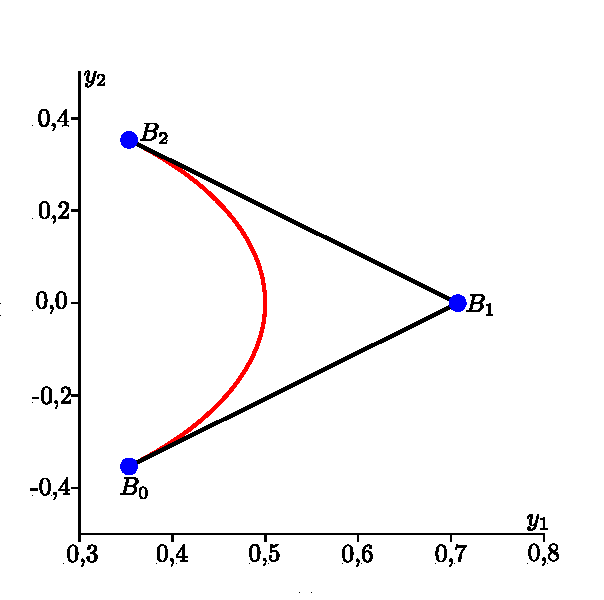
\includegraphics[scale=0.7,trim=0.6cm 0cm 0cm 0cm, clip=true]{Imagens/Cap3/cilindro_circ_ini.pdf}}  \ \ \
	\subfloat[\label{fig:cilindro_circ_ref}Curva refinada e rede de pontos de controle]{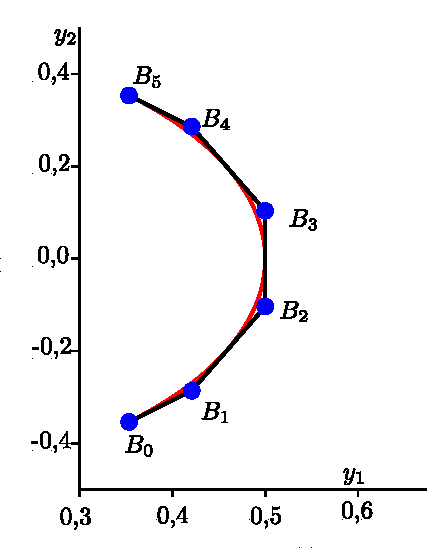
\includegraphics[scale=0.7,trim=0cm 0cm 0cm 1cm, clip=true]{Imagens/Cap3/cilindro_circ_ref.pdf}} \\ 
	\caption{Cilindro: Obtenção da circunferência}
	\label{fig:cilindro_geo0}
\end{figure}


Dando continuidade a descrição exemplificativa da geometria do \textit{patch} $P_0$, gerou-se uma curva na direção paramétrica $\xsi$ que define o contorno direito do domínio. A curva é definida considerando o vetor de \textit{knots} atualizado $\Xsi=\left[0,0,0,1/4,1/2,3/4,1,1,1\right]$, e,  consiste em uma reta cujas coordenadas de suas extremidades inicial e final são: $\pos_0 =[2,-2,0]$ e $\pos_1 =[2, 2 ,0]$, respectivamente. Os $6$ pontos de controle são distribuídos sobre a reta através de um espaçamento não uniforme: nas extremidades, a distância entre pontos consecutivos corresponde à metade do espaçamento adotado no interior, enquanto a região central é subdividida uniformemente, conforme pode ser observado na Fig. \ref{fig:cilindro_pc_superficie}. Essa distribuição não uniforme dos pontos de controle, proporcionada para essa discretização, uma distribuição uniforme das células mapeadas no espaço físico. Para essa curva, os todos os pesos foram definidos como $1$.

A superfície do domínio foi gerada discretizando-se a direção $\eta$ do espaço paramétrico. Para isso, os $m+1$ pontos de controle nessa direção foram posicionados ao longo das retas que conectam os pontos de controle da primeira camada (circunferência) aos da última camada (reta). A distribuição desses pontos seguiu uma progressão geométrica, de modo que as células menores se localizassem próximas ao cilindro, captando adequadamente os efeitos de camada limite. Para garantir que essa distribuição também se refletisse nas células mapeadas para o espaço físico, aplicou-se um fator de correção aos pontos de controle intermediários $B_{i,1}$ e $B_{i,m-1}$, para $i = 0, 1, \dots , n$, deslocando-os em direção aos pontos de controle das extremidades.

A fim de exemplificar a geração da superfície, adotou-se a discretização mínima necessária, utilizando apenas três pontos de controle na direção $\eta$, para o emprego de funções quadráticas e vetor de \textit{knots} aberto $\mathcal{H}=[0,0,0,1,1,1]$, conforme pode-se observar na Fig. \ref{fig:cilindro_pc_superficie}. Na fig. \ref{fig:cilindro_malhafisica_superficie} apresentam-se as células mapeadas do espaço paramétrico para o espaço físico. Salienta-se que os pontos de controle obtidos nessa etapa foram definidos com peso unitário.

Para a simulação numérica apresentada na sequência a quantidade de pontos de controle na direção $\eta$ foi definida em função da necessidade de discretização para o problema. Para um vetor de \textit{knots} abertos com coordenadas interiores de multiplicidade unitária, a quantidade de células ($ncel$) está relacionada a quantidade de pontos de controle por $ncel = npc-deg$, sendo $npc$ o número de pontos de controle e $deg$ o grau das funções na direção paramétrica em questão.

\begin{figure}[!t]
	\centering
	\subfloat[\label{fig:cilindro_pc_superficie} Rede de pontos de controle superfície]{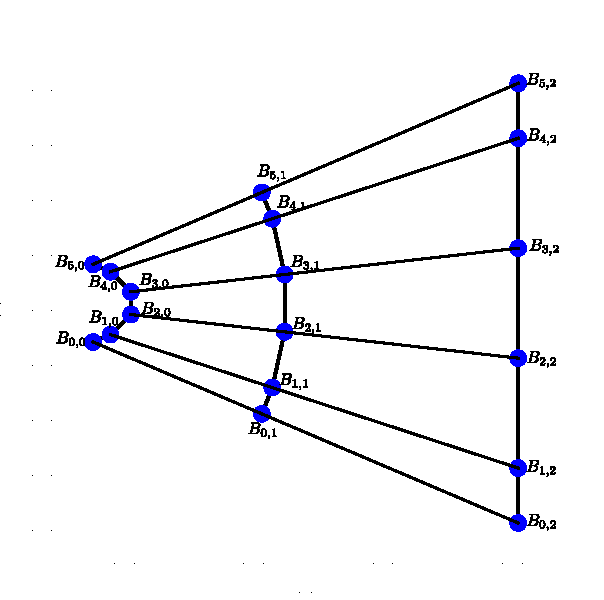
\includegraphics[scale=0.8,trim=0cm 0cm 0cm 1cm, clip=true]{Imagens/Cap3/cilindro_pc_superficie.pdf}}   
	\subfloat[\label{fig:cilindro_malhafisica_superficie} Malha física]{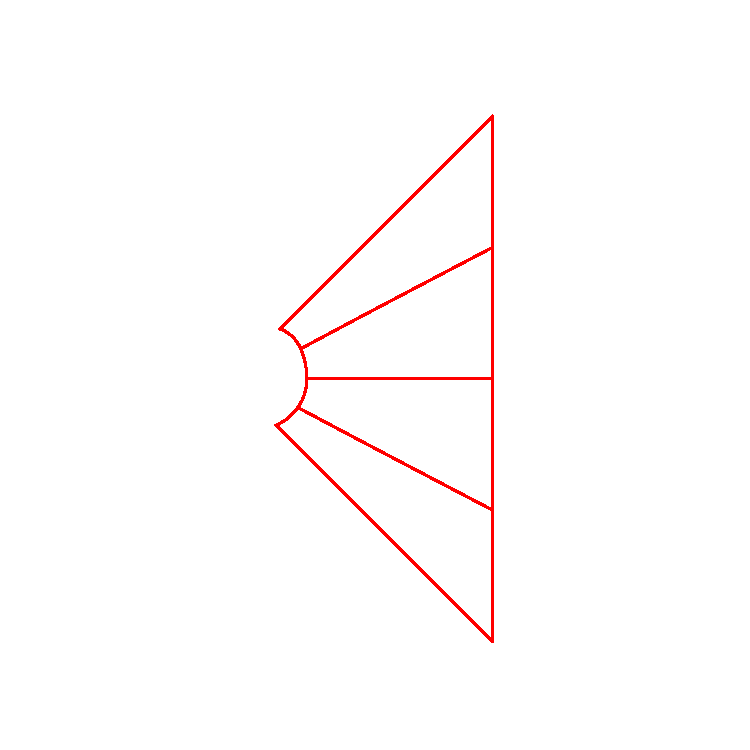
\includegraphics[scale=0.8,trim=3cm 1.5cm 3cm 1cm, clip=true]{Imagens/Cap3/cilindro_malhafisica_superficie.pdf}} 
	\caption{Cilindro: Obtenção da superfície}
	\label{fig:cilindro_geo1}
\end{figure}

Por fim, para a geração do sólido NURBS, com apenas uma camada de células na direção paramétrica $\zeta$, correspondente à direção $y_3$ do espaço físico deste problema, foram utilizadas funções quadráticas, um vetor de \textit{knots} aberto $\mathcal{Z} = \left[0,0,0,1,1,1\right]$, assim como pontos de controle distribuídos uniformemente e de peso unitário. Na Fig. \ref{fig:cilindro_pc_solido} pode-se observar a rede de pontos de controle resultante, na qual a nomenclatura dos pontos foi omitida para facilitar a visualização. Na fig. \ref{fig:cilindro_malhafisica_solido} apresenta-se a malha física derivada da discretização exemplificativa do \textit{patch} $P_0$.

\begin{figure}[!t]
	\centering
	\subfloat[\label{fig:cilindro_pc_solido}Rede de pontos de controle sólido]{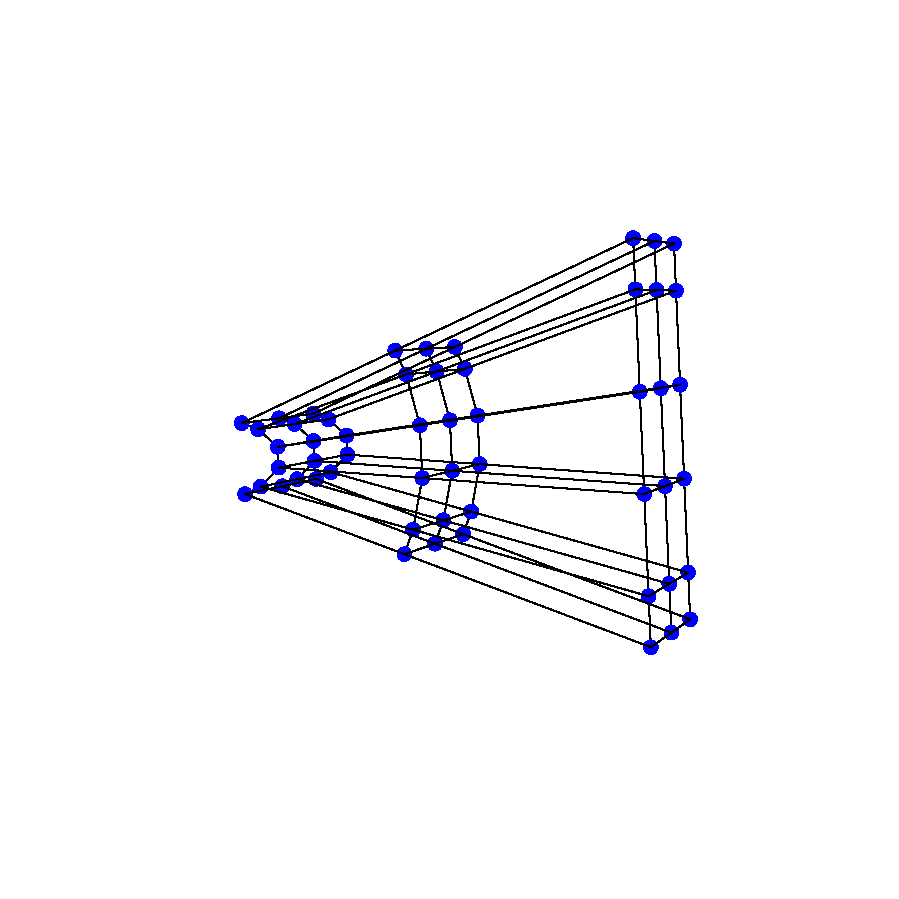
\includegraphics[scale=0.8,trim=2cm 3cm 3cm 3cm, clip=true]{Imagens/Cap3/cilindro_pc_solido.pdf}}   \ \ 
	\subfloat[\label{fig:cilindro_malhafisica_solido}Malha física sólido]{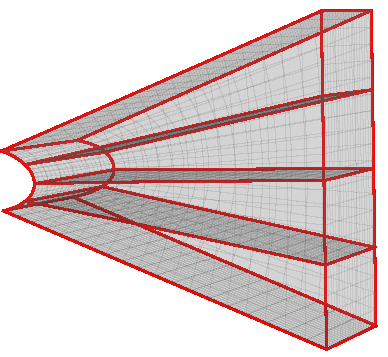
\includegraphics[scale=1.0,trim=0cm 0cm 0cm 0cm, clip=true]{Imagens/Cap3/cilindro_malhafisica_solido.pdf}} 
	\caption{Cilindro: Obtenção do sólido}
	\label{fig:cilindro_geo2}
\end{figure}

Para os \textit{patches} $P_1$, $P_2$ e $P_3$, utiliza-se a mesma parametrização de $P_0$, obtendo-se seus pontos de controle por rotação dos pontos de controle de $P_0$, de modo que cada um seja ajustado ao quadrante do cilindro correspondente.

Para a geração dos demais \textit{patches} retangulares, $P_4$ à $P_{11}$, definiu-se a direção paramétrica $\xsi$ respectiva à direção física $y_1$, $\eta$ correspondente à $y_2$ e $\zeta$ à $y_3$. A quantidade de pontos de controle em cada direção foi definida a partir do número de células desejadas para a análise numérica. Considerando o exposto anterior para o \textit{patch} $P_0$, a distribuição dos pontos de controle foi realizada de forma a se obter células físicas igualmente espaçadas, ou, arranjadas com um espaçamento que segue uma distribuição geométrica. Os pontos de controle foram definidos com peso unitário. Os vetores de \textit{knots} são abertos e com espaçamento interior subdividido de maneira uniforme. As funções NURBS utilizadas foram quadráticas. 

Destaca-se que na discretização de todos os \textit{patches} é necessário garantir uma parametrização idêntica nos planos que apresentam fronteira com outro \textit{patch}.


\subsubsection {Análise numérica}

Conforme exposto na Subseção \ref{capitulo:Cap2:VerApl:Cilindo} o estudo do problema de escoamento sobre um cilindro proporciona avaliar se o modelo computacional implementado é capaz de reproduzir os fenômenos relacionados à formação e desprendimentos de vórtices, além de propiciar a validação do código através da comparação dos coeficientes aerodinâmicos medidos ao longo do tempo com referências bibliográficas disponíveis na literatura especializada. Visando a verificação do código de IGA com células 3D analisa-se o problema do escoamento sobre o cilindro para $\Reynolds = 40$, $\Reynolds = 100$, e, $\Reynolds = 1000$.

O domínio do problema simulado é um volume retangular discretizado em função do diâmetro do cilindro e é apresentado na Fig. \ref{fig:cilindro_geometria3d}. A dimensão $t$ na direção $y_3$ é equivalente à $0,01D$. Aplica-se um perfil de velocidade constante na entrada do domínio, $\velocity=[u_\infty,0,0]$, e condições de parede lisa são atribuídas às paredes superior e inferior, enquanto que para as frontal e dos fundos condições de simetria são aplicadas.

A malha isogeométrica utilizada é apresentada na Fig. \ref{fig:cilindro_malha3d} e na Tab. \ref{tab:cilindro_discretização_patches} pode-se observar a quantidade de pontos de controle em cada uma das direções paramétricas utilizados na discretização de cada um dos \textit{patches} que compõe a malha, resultando em 30228 pontos de controle e 8728 células físicas.


\begin{figure}[!htb]
	\centering
	\subfloat[Cilindro: Geometria e condições de contorno\label{fig:cilindro_geometria3d}]{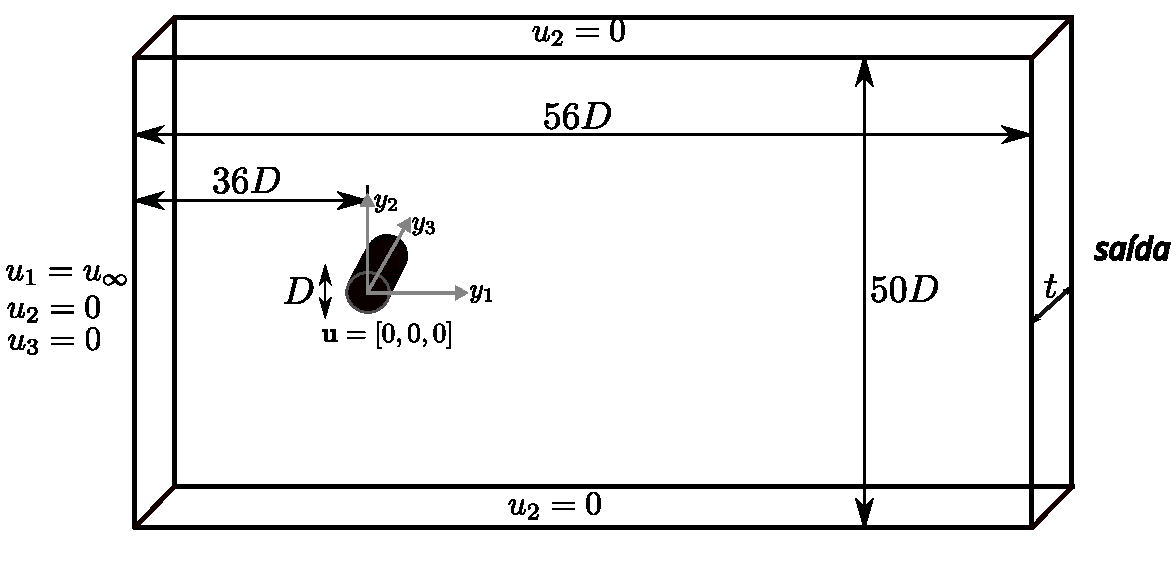
\includegraphics[scale=0.6,trim=0cm 0cm 0cm 0cm, clip=true]{Imagens/Cap3/cilindro_geometria3d.pdf}}\\
	\subfloat[Discretização espacial - plano $y_1$$y_2$\label{fig:cilindro_malha3d}]{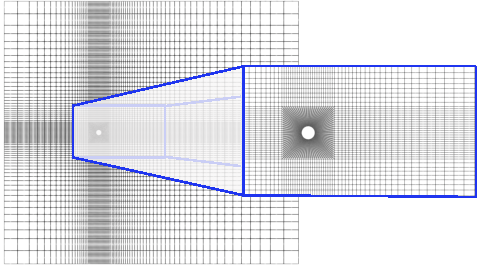
\includegraphics[trim=0cm 0cm 0cm 0cm,clip,scale=1.2]{Imagens/Cap3/cilindro_malha.pdf}}
	\caption{Cilindro: Malha de células físicas}
\end{figure}

\begin{table}[h]
	\caption{Cilindro: Número de pontos de controle por \textit{patch}}
	\centering
	\begin{minipage}{0.49\textwidth}
		\centering
		\begin{tabular}{|c | c | c| c|} 
		\hline
		\textit{Patch} & $\xsi$ & $\eta$ & $\zeta$\\ 
		\hline
		0 & 26 & 34 & 3\\
		\hline
		1 & 26 & 34 & 3\\
		\hline
		2 & 26 & 34 & 3\\
		\hline
		3 & 26 & 34 & 3\\
		\hline
		4 & 20 & 28 & 3\\
		\hline
		5 & 26 & 28 & 3\\ 
		\hline
		\end{tabular}
	\end{minipage}%
	\hspace{-3cm}  % valor negativo diminui distância
	\begin{minipage}{0.49\textwidth}
		\centering
		\begin{tabular}{|c | c | c| c|} 
		\hline
		\textit{Patch} & $\xsi$ & $\eta$ & $\zeta$\\ 
		\hline
		6 & 42 & 28 & 3\\
		\hline
		7 & 20 & 26 & 3\\
		\hline
		8 & 42 & 26 & 3\\
		\hline
		9 & 20 & 28 & 3\\
		\hline
		10 & 26 & 28 & 3\\
		\hline
		11 & 42 & 28 & 3\\ 
		\hline
		\end{tabular}
		\label{tab:cilindro_discretização_patches}
	\end{minipage}
\end{table}


O problema é simulado para um velocidade de entrada $u_{\infty} = 1,0$, $\rho = 1,0$, $\timeStep = 0,05$, e $\specRadius = 0,5$, sendo a viscosidade variada de acordo com o número de Reynolds desejado.  Calculam-se os coeficientes aerodinâmicos, $C_{D}$ e $C_{L}$, a partir das definições de forças de arrasto e de sustentação apresentadas respectivamente nas Eq. \ref{eq:F_D} e Eq.\ref{eq:F_L}, através das seguintes equações:

\begin{align}
	C_D = \frac{F_D}{0,5\density \lVert \velocinfty \lVert^{2} L t},
\end{align}

\begin{align}
	C_L = \frac{F_L}{0,5\density \lVert \velocinfty \lVert^{2} L t},
\end{align}.


Nas Figs. \ref{fig:cilindro_cd3d} e \ref{fig:cilindro_cl3d}, apresenta-se a variação ao longo do tempo dos coeficientes aerodinâmicos $C_{D}$ e $C_{L}$. Os valores do coeficiente de arrasto médio obtidos com a malha isogeométrica com células 3d foram: $C_{Dmed} = 1,54$ para $\Reynolds = 40$, $C_{Dmed} = 1,36$ para $\Reynolds = 100$ e $C_{Dmed} = 1,49$ para $\Reynolds = 1000$. Ressalta-se, que apesar dos valores de $C_{Dmed}$ estarem bem próximos aos da simulação com MEF tradicional da Subseção \ref{capitulo:Cap2:VerApl:Cilindo}, para as análises utilizando IGA, foram necessários mais passos de tempo para o início do processo de desprendimento de vórtices, nos casos de $\Reynolds = 100$ e $\Reynolds = 1000$. 

\begin{figure}[!htb]
	\centering
	\subfloat[\label{fig:cilindro_cd3d}Coeficiente de arrasto $ C_D$]{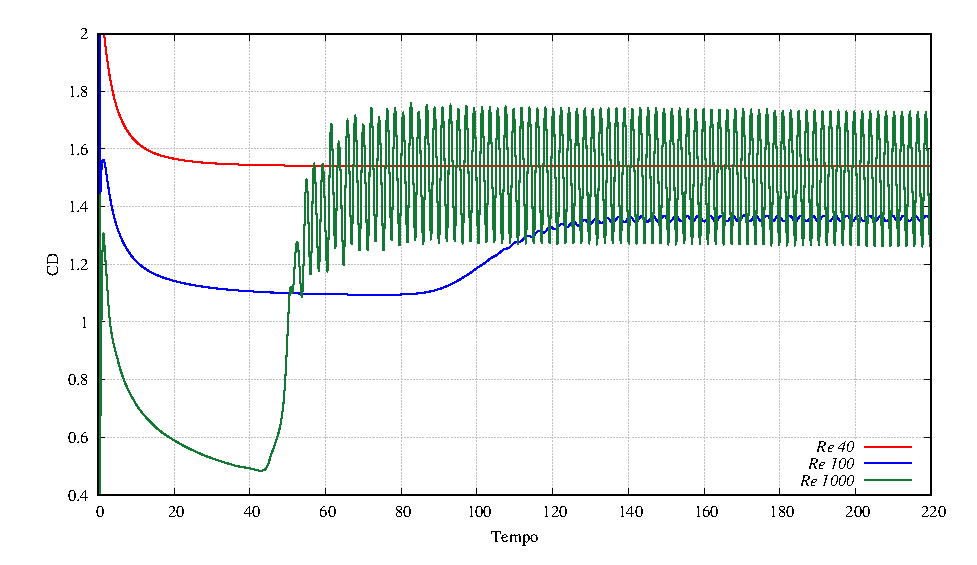
\includegraphics[scale=0.8,trim=0cm 0cm 0cm 0cm, clip=true]{Imagens/Cap3/cilindro_CD.eps}}  \\
	\subfloat[\label{fig:cilindro_cl3d}Coeficiente de sustentação $C_L$]{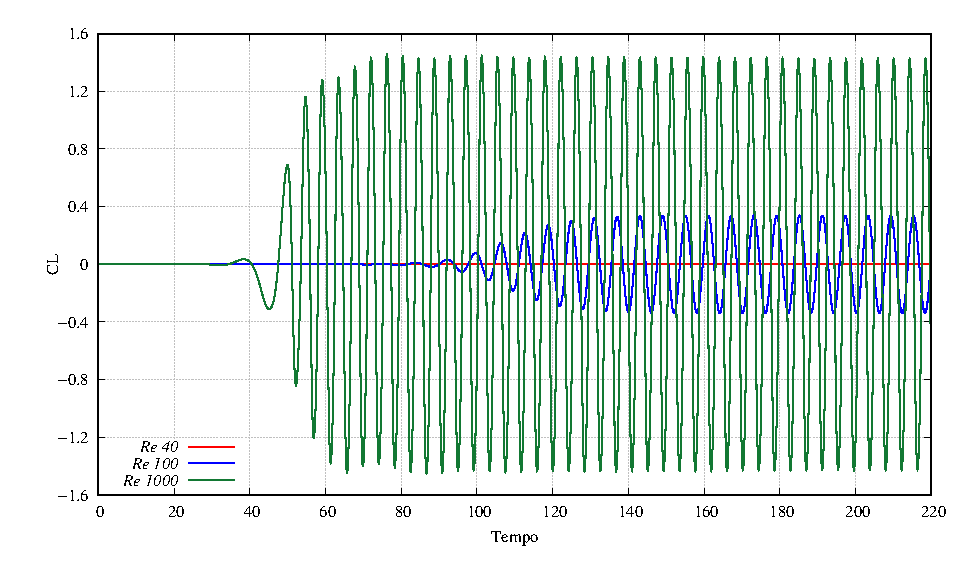
\includegraphics[scale=0.8,trim=0cm 0cm 0cm 0cm, clip=true]{Imagens/Cap3/cilindro_CL.eps}}\\ 
	{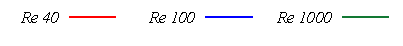
\includegraphics[scale=1.3]{Imagens/Cap3/Legenda.pdf}}
	\caption{Cilindro: Coeficientes aerodinâmicos }
	\label{fig:cilindro_coeficientes3d}
\end{figure}

Nas Fig. \ref{fig:cilindro_iga_camposVel} e Fig. \ref{fig:cilindro_iga_camposPressao} são apresentados os campos de velocidade e pressão ao longo de um ciclo de desprendimento de vórtices para $\Reynolds = 1000$.


\begin{figure}[htb!]
	\centering
	\subfloat[$T_n$]{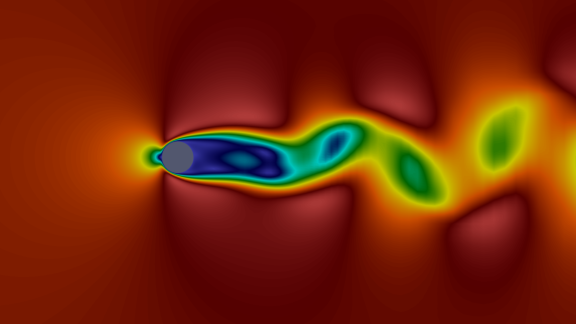
\includegraphics[scale=0.7,trim=0cm 0cm 0cm 0cm, clip=true]{Imagens/Cap3/cilindro_vel_tn.pdf}} \
	\subfloat[$T_n + T_n/6$]{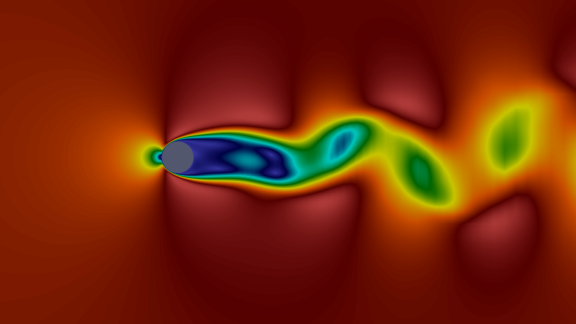
\includegraphics[scale=0.7,trim=0cm 0cm 0cm 0cm, clip=true]{Imagens/Cap3/cilindro_vel_tn6.pdf}} \\
	\subfloat[$T_n + T_n/3$]{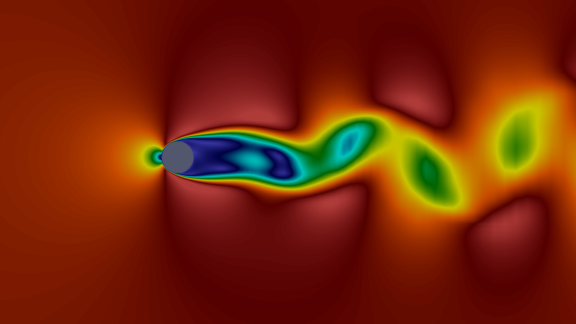
\includegraphics[scale=0.7,trim=0cm 0cm 0cm 0cm, clip=true]{Imagens/Cap3/cilindro_vel_tn3.pdf}} \
	\subfloat[$T_n + T_n/2$]{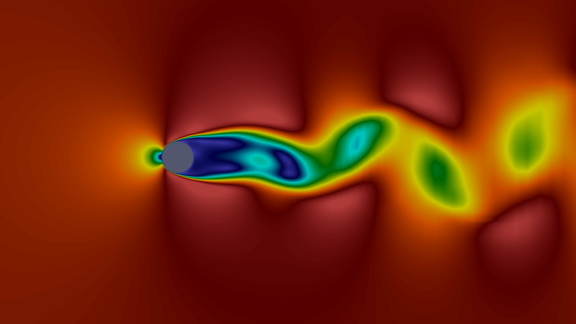
\includegraphics[scale=0.7,trim=0cm 0cm 0cm 0cm, clip=true]{Imagens/Cap3/cilindro_vel_tn2.pdf}} \\
	\subfloat[$T_n + 2T_n/3$]{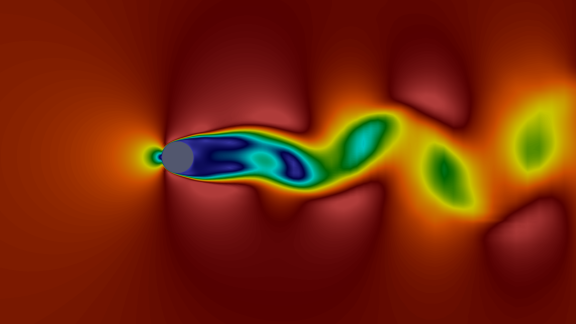
\includegraphics[scale=0.7,trim=0cm 0cm 0cm 0cm, clip=true]{Imagens/Cap3/cilindro_vel_2tn3.pdf}} \
	\subfloat[$T_n + 5T_n/6$]{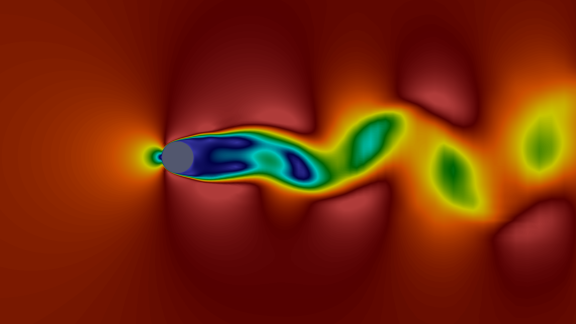
\includegraphics[scale=0.7,trim=0cm 0cm 0cm 0cm, clip=true]{Imagens/Cap3/cilindro_vel_5tn6.pdf}} \\
	{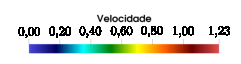
\includegraphics[trim=0cm 0cm 0cm 0cm,clip=true,scale=1.4]{Imagens/Cap3/cilindro_vel_legenda.pdf}} \\
	\caption{Cilindro: Campos de velocidade para $\Reynolds = 1000$ - plano $y_1$$y_2$}
	\label{fig:cilindro_iga_camposVel}
\end{figure}

\begin{figure}[htb!]
	\centering
	\subfloat[$T_n$]{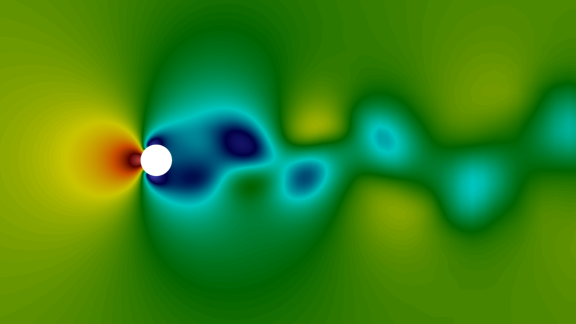
\includegraphics[scale=0.7,trim=0cm 0cm 0cm 0cm, clip=true]{Imagens/Cap3/cilindro_press_tn.pdf}} \
	\subfloat[$T_n + T_n/6$]{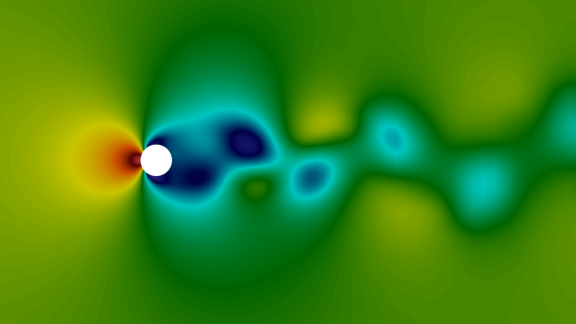
\includegraphics[scale=0.7,trim=0cm 0cm 0cm 0cm, clip=true]{Imagens/Cap3/cilindro_press_tn6.pdf}} \\
	\subfloat[$T_n + T_n/3$]{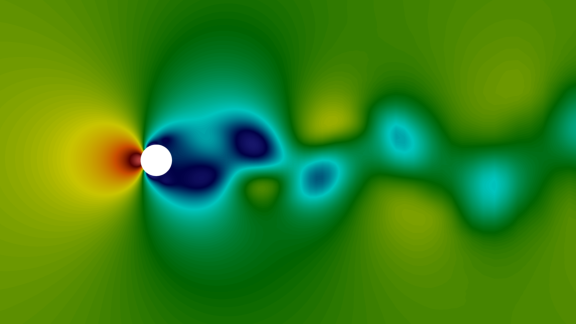
\includegraphics[scale=0.7,trim=0cm 0cm 0cm 0cm, clip=true]{Imagens/Cap3/cilindro_press_tn3.pdf}} \
	\subfloat[$T_n + T_n/2$]{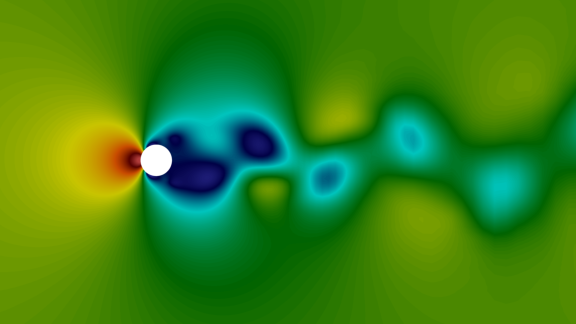
\includegraphics[scale=0.7,trim=0cm 0cm 0cm 0cm, clip=true]{Imagens/Cap3/cilindro_press_tn2.pdf}} \\
	\subfloat[$T_n + 2T_n/3$]{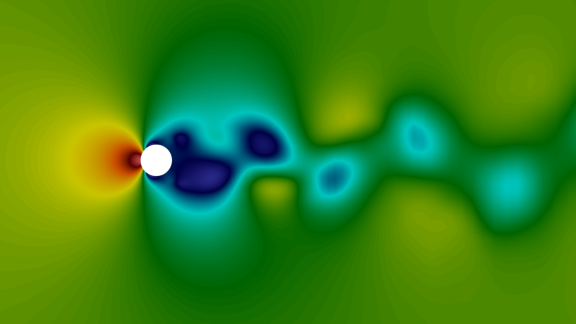
\includegraphics[scale=0.7,trim=0cm 0cm 0cm 0cm, clip=true]{Imagens/Cap3/cilindro_press_2tn3.pdf}} \
	\subfloat[$T_n + 5T_n/6$]{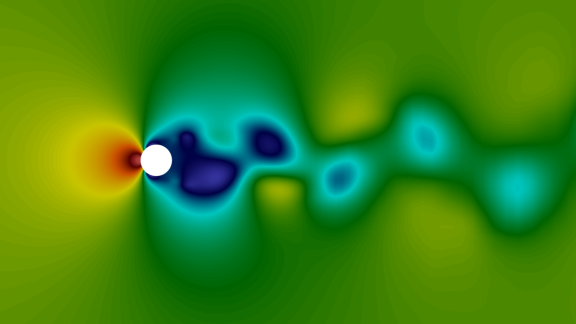
\includegraphics[scale=0.7,trim=0cm 0cm 0cm 0cm, clip=true]{Imagens/Cap3/cilindro_press_5tn6.pdf}} \\
	{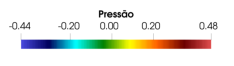
\includegraphics[trim=0cm 0cm 0cm 0cm,clip=true,scale=1.4]{Imagens/Cap3/cilindro_press_legenda.pdf}} \\
	\caption{Cilindro: Campos de pressão para $\Reynolds = 1000$ - plano $y_1$$y_2$}
	\label{fig:cilindro_iga_camposPressao}
\end{figure}


\subsection {Escoamento em um canal com degrau}

O problema de escoamento em canal com degrau consiste na aplicação de um perfil de velocidade parabólico na entrada de um canal, o qual caracteriza-se pela presença de um degrau próximo a entrada do escoamento. A existência do degrau acarreta na formação de um vórtice de recirculação, chamado aqui de vórtice primário, o qual aumenta de tamanho, a medida que se eleva o número de Reynolds do escoamento. A dimensão do vórtice primário, para diferentes números de Reynolds, será alvo de avaliação nessa seção, através da análise comparativa deste dado com bibliografias de referência.

Na Fig.\ref{fig:degrau_geometria} apresenta-se a configuração geral da geometria do canal, que foi discretizado através do uso de células isogeométricas 3d definidas dentro de cinco \textit{patches} que descrevem o domínio do problema. As dimensões do canal são: $h = 1,0m$, $s = 0,94m$, $x_{e}= 1,0m$, $x_{f}= 15m$ e $x_{t} = 30m$. A profundidade do canal adotada, na direção $y_3$, é equivalente a $0,1m$. Devido a pequena dimensão definida em $y_3$ a simulação numérica realizada é caracterizada como um escoamento em domínio bidimensional.

\begin{figure}[htb!]
	\centering
	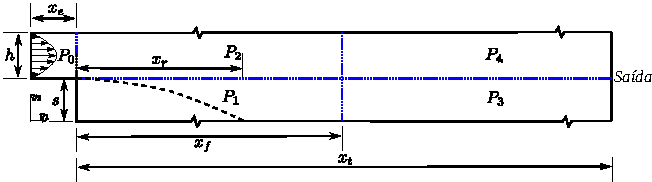
\includegraphics[scale=1.2,trim=0cm 0cm 0cm 0cm, clip=true]{Imagens/Cap3/degrau_geometria.pdf}
	\caption{Degrau: Geometria - plano $y_1$$y_2$}
	\label{fig:degrau_geometria}
\end{figure}

Para a geração da geometria NURBS, os 5 \textit{patches}, denominados $P_{0},P_{1},P_{2},P_{3}$ e $P_{4}$, são discretizados em todas as direções paramétricas com funções base quadráticas e com vetores de \textit{knots} abertos de coordenadas paramétricas igualmente espaçados em seu interior. Os pontos de controle para os \textit{patches} $P_0$, $P_1$ e $P_2$ foram distribuídos no espaço físico, direções $y_1$, $y_2$ e $y_3$, de maneira a se obter células igualmente espaçadas. Ressalta-se, que o número de células está relacionado a quantidade de pontos de controle por $ncel = npc-deg$.
Para os \textit{patches} $P_3$ e $P_4$, na direção do espaço físico $y_2$ e $y_3$, os pontos de controle são posicionadas de maneira a gerar células uniformes, e, na direção $y_1$, são distribuídos de maneira a se obter células em progressão geométrica, aumentando de tamanho no sentido do contorno de saída, conforme pode ser observado na Fig. \ref{fig:degrau_malha}. Na Tab. \ref{tab:degrau_discretização_patches} apresenta-se o número de pontos de controle em cada direção paramétrica para cada \textit{patch}, resultando em 17640 pontos de controle e 4800 células.

\begin{figure}[htb!]
	\centering
	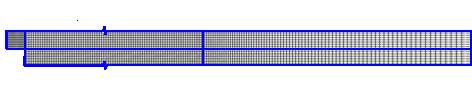
\includegraphics[scale=2.0,trim=0cm 0.1cm 0cm 0cm, clip=true]{Imagens/Cap3/degrau_malha.pdf}
		\vspace{-0.5cm} 
	\caption{Degrau: Malha de células físicas - plano $y_1$$y_2$}
	\label{fig:degrau_malha}
\end{figure}

\begin{center}
	\begin{table}[h!]
		\caption{Degrau: Número de pontos de controle por \textit{patch}}
		\centering
		\begin{tabular}{|c | c | c| c|} 
			\hline
			\textit{Patch} & $\xsi$ & $\eta$ & $\zeta$ \\ 
			\hline
			0 & 22 & 12 & 3 \\ 
			\hline
			1 & 152 & 12 & 3\\
			\hline
			2 & 152 & 12 & 3\\
			\hline
			3 & 82 & 12 & 3\\
			\hline
			4 & 82 & 12 & 3\\
			\hline
		\end{tabular}
		\label{tab:degrau_discretização_patches}
	\end{table}
\end{center}

Para a simulação numérica, aplicou-se condição de aderência nos contornos contidos nos planos $y_1$$y_3$ e $y_1$$y_3$, exceto naqueles com condições de entrada ou de saída. Nos contornos contidos nos planos $y_1$$y_2$ aplicou-se condição de simetria. O perfil parabólico adotado na entrada do domínio é descrito pela seguinte equação:

\begin{align}
u_{1} = V_{max} \left(1-\left(\frac{\left(y_2-s\right)-h/2}{h/2}\right)^{2}\right),
\end{align}

\noindent com velocidade $V_{max} = 10 m/s$ e $u_{2} = u_{3} = 0$ nesse contorno.

O escoamento sobre o degrau é caracterizado por produzir áreas de recirculação onde o fluido se separa e forma vórtices. A distância entre o degrau e o ponto de recolamento do vórtice principal, $x_{r}$, é uma das principais características verificadas nesse problema. A dimensão dos vórtices varia em função do número de $\Reynolds$, o qual é calculado de acordo com \citeonline {ArmalyDP:1983}, por:

\begin{align}
\Reynolds =\frac{\rho\left(\frac{2V_{max}}{3}\right)2h}{\viscosity}.
\end{align}

Foram selecionados três diferentes número de Reynolds para as análises: $\Reynolds = 100$, $\Reynolds = 400$ e $\Reynolds = 800$, os quais são obtidos a partir da variação da viscosidade do fluido. Considerou-se  $\rho = 1kg/m^{3}$, $\timeStep = 0,05s$, e $\specRadius = 0,5$.

De acordo com os experimentos realizados por \citeonline{ArmalyDP:1983}, as medições do comprimento do vórtice primário, logo a jusante do degrau na parte inferior, identificam o regime do escoamento como laminar ($\Reynolds < 1200$), transiente ($1200 < \Reynolds < 6600$) e turbulento ($\Reynolds > 6600$). Além disso, o autor constatou em seus ensaios que para $\Reynolds < 400$ o escoamento é predominantemente bidimensional, enquanto que para Reynolds superiores,  o escoamento apresenta regiões de comportamento tridimensional. 

\citeonline{ArmalyDP:1983} em suas análises constatou o surgimento de uma bolha de separação adicional ao longo do piso do canal, a jusante da separação primária, a qual desaparece para $\Reynolds > 2300$. Outra região de separação secundária também foi observada ao longo da parede superior, a jusante do degrau, desenvolvendo-se a partir de Re 400 e permanecendo durante todo o regime de transição.

Na Fig. \ref{fig:degrau_comprimento_vortice_principal} são apresentados os comprimentos de recolamento do vórtice primário adimensionalizados ($x_{r}/s$) obtidos nesse trabalho, juntamente com os valores adaptados dos ensaios experimentais de \citeonline{ArmalyDP:1983} e os resultados de análises 2d e 3d de \citeonline{WilliamsB:1999}. Com essa figura é possível observar que a medida que o número de Reynolds aumenta, os resultados obtidos do presente estudo se afastam dos valores de referência respectivos ao estudo experimental e da simulação tridimensional. Este fato ocorre visto que o ensaio experimental foi realizado em um canal com $2m$ profundidade na direção $y_3$, enquanto que a simulação atual conta com apenas uma célula nessa direção, sendo então incapaz de captar os fenômenos tridimensionais que ocorrem a medida que o número de Reynolds cresce. 

Na Fig.\ref {fig:degrau_campos_velocidade_Re100} pode-se observar o campo de velocidade para o domínio completo e para a região do vórtice primário para $\Reynolds = 100$, enquanto que na Fig. \ref {fig:degrau_campos_velocidade_Re400} e na Fig. \ref {fig:degrau_campos_velocidade_Re800} são apresentados para $\Reynolds = 400$ e $\Reynolds = 800$ respectivamente. Para $\Reynolds = 800$ constatou-se a formação de um vórtice secundário na parede superior, conforme havia sido relatado pelos autores previamente citados, conforme pode ser observado na Fig. \ref{fig:degrau_vor_sec_re800}.

Por fim, na Fig. \ref{fig:degrau_campos_pressao} é possível observa-se os campos de pressão para todos os números de Reynolds simulados.

\begin{figure}[htb!]
	\centering
	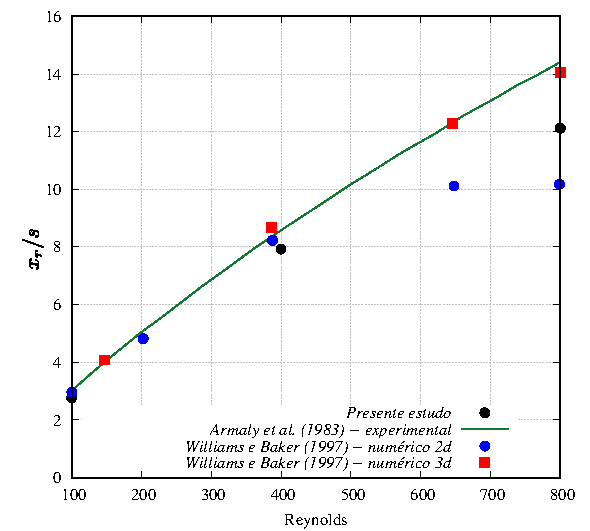
\includegraphics[scale=1.2,trim=0cm 0cm 0cm 0cm, clip=true]{Imagens/Cap3/degrau_vort_prim.pdf}
	\caption{Degrau: Comprimento do vórtice principal}
	\label{fig:degrau_comprimento_vortice_principal}
\end{figure}

\begin{figure}[!htb]
	\centering
	\subfloat[\label{fig:degrau_vel_re100} Domínio Completo]{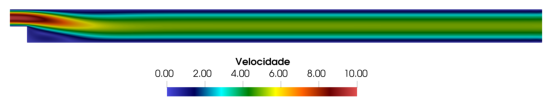
\includegraphics[scale=1.55,trim=0.0cm 0cm 0cm 0cm, clip=true]{Imagens/Cap3/degrau_vel_100.pdf}} \\
	\subfloat[\label{fig:degrau_vor_re100} Vórtice primário ]{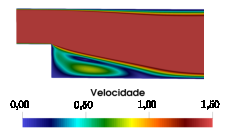
\includegraphics[scale=1.55,trim=0.0cm 0cm 0cm 0cm, clip=true]{Imagens/Cap3/degrau_vor_100.pdf}}
	\caption{Degrau: Campos de velocidade para $\Reynolds = 100$ }
	\label{fig:degrau_campos_velocidade_Re100}
\end{figure}

\begin{figure}[!htb]
	\centering
	\subfloat[\label{fig:degrau_vel_re400} Domínio Completo]{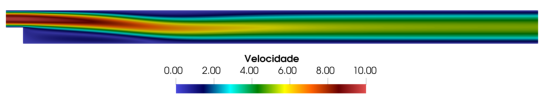
\includegraphics[scale=1.55,trim=0.0cm 0cm 0cm 0cm, clip=true]{Imagens/Cap3/degrau_vel_400.pdf}} \\
	\subfloat[\label{fig:degrau_vor_re400} Vórtice primário ]{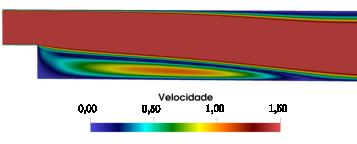
\includegraphics[scale=1.55,trim=0.0cm 0cm 0cm 0cm, clip=true]{Imagens/Cap3/degrau_vor_400.pdf}}
	\caption{Degrau: Campos de velocidade para $\Reynolds = 400$ }
	\label{fig:degrau_campos_velocidade_Re400}
\end{figure}

\begin{figure}[!htb]
	\centering
	\subfloat[\label{fig:degrau_vel_re800} Domínio Completo]{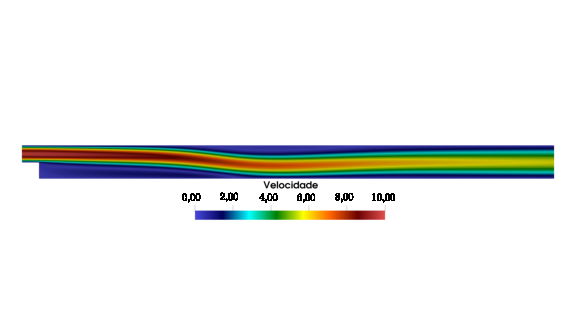
\includegraphics[scale=1.55,trim=0.0cm 1.5cm 0cm 1.5cm, clip=true]{Imagens/Cap3/degrau_vel_800.pdf}} \\
	\subfloat[\label{fig:degrau_vor_re800} Vórtice primário ]{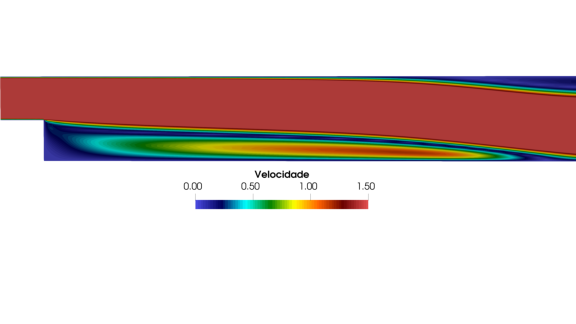
\includegraphics[scale=1.55,trim=0.0cm 1.7cm 0cm 1.5cm, clip=true]{Imagens/Cap3/degrau_vor_800.pdf}}\\
	\subfloat[\label{fig:degrau_vor_sec_re800} Vórtice secundário ]{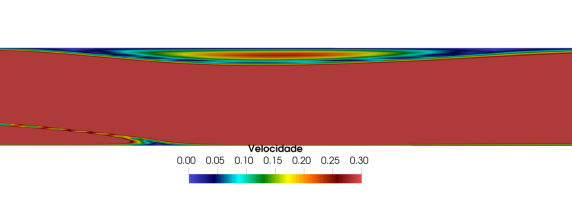
\includegraphics[scale=1.4,trim=0.0cm 0.5cm 0cm 0.7cm, clip=true]{Imagens/Cap3/degrau_vor_sec_800.pdf}}
	\caption{Degrau: Campos de velocidade para $\Reynolds = 800$ }
	\label{fig:degrau_campos_velocidade_Re800}
\end{figure}


\begin{figure}[!htb]
	\centering
	\subfloat[\label{fig:degrau_press_re100} $\Reynolds= 100$]{
\includegraphics[scale=1.5,trim=0cm 0cm 0cm 0cm, clip=true]{Imagens/Cap3/degrau_press_100.pdf}} \\
	\subfloat[\label{fig:degrau_press_re400} $\Reynolds= 400$]{\includegraphics[scale=1.5,trim=0cm 0cm 0cm 0cm, clip=true]{Imagens/Cap3/degrau_press_400.pdf}} \\
	\subfloat[\label{fig:degrau_press_re800} $\Reynolds= 800$]{\includegraphics[scale=1.5,trim=0cm 0cm 0cm 0cm, clip=true]{Imagens/Cap3/degrau_press_800.pdf}}
	\caption{Degrau: Campos de pressão }
	\label{fig:degrau_campos_pressao}
\end{figure}

\end{document}

\end{document}
